% !TEX program = lualatex
\documentclass[12pt,a4paper]{article}

%==================== Preamble ====================
% --- Font and Typography ---
\usepackage{fontspec}
\setmainfont{TeX Gyre Termes}[Ligatures=TeX]

% --- Micro-typography ---
\usepackage{microtype}

% --- Page Geometry ---
\usepackage{geometry}
\geometry{margin=1.05in}

% --- Line Spacing and Paragraphs ---
\usepackage{setspace}
\usepackage{parskip}

% --- Section Formatting ---
\usepackage{titlesec}
\titleformat{\section}{\Large\bfseries}{\thesection.}{0.6em}{}
\titleformat{\subsection}{\large\bfseries}{\thesubsection.}{0.6em}{}
\titleformat{\subsubsection}{\normalsize\bfseries\itshape}{\thesubsubsection.}{0.5em}{}

% --- Math Packages (load in logical order) ---
\usepackage{amsmath,amssymb,amsthm,mathtools,bm}
\usepackage{physics}
\usepackage{tensor}
\usepackage{siunitx}
\usepackage{upgreek}
\usepackage{mathrsfs} % for \mathscr

% --- Graphics and Tables ---
\usepackage{graphicx}
\usepackage{float}
\usepackage{subcaption}
\usepackage{booktabs}
\usepackage{enumitem}

% --- Color ---
\usepackage{xcolor}

% --- PGF/TikZ and PGFPlots ---
\usepackage{pgfplots}
\pgfplotsset{compat=1.18}
\usepackage{tikz}
\usetikzlibrary{
  arrows.meta,
  positioning,
  calc,
  decorations.markings,
  decorations.pathmorphing,
  backgrounds,
  3d,
  angles,
  quotes
}

% --- Hyperref (load near end, before natbib) ---
\usepackage[
  colorlinks=true,
  linkcolor=blue,
  citecolor=teal,
  urlcolor=magenta,
  pdfencoding=auto
]{hyperref}

% --- Bibliography (load after hyperref) ---
\usepackage[authoryear]{natbib}
\bibpunct{(}{)}{;}{a}{}{,}

% Theorem environments
\numberwithin{equation}{section}
\newtheorem{definition}{Definition}[section]
\newtheorem{assumption}{Assumption}[section]
\newtheorem{lemma}{Lemma}[section]
\newtheorem{proposition}{Proposition}[section]
\newtheorem{theorem}{Theorem}[section]
\theoremstyle{remark}
\newtheorem{remark}{Remark}[section]
\theoremstyle{definition}
\newtheorem{example}{Example}[section]
\newtheorem{corollary}{Corollary}[section]

% Handy macros
\newcommand{\M}{\mathbb{M}}
\newcommand{\R}{\mathbb{R}}
\newcommand{\C}{\mathbb{C}}
\newcommand{\ii}{\mathrm{i}}
\newcommand{\ee}{\mathrm{e}}
\newcommand{\h}{\hbar}
\newcommand{\lap}{\Delta}
\newcommand{\cl}{\mathrm{cl}}
\newcommand{\q}{\mathrm{q}}
\newcommand{\sgn}{\operatorname{sgn}}
\DeclareMathOperator{\supp}{supp}
\DeclareMathOperator{\argmin}{arg\,min}
\newcommand{\pboxtimes}{\mathbin{\boxtimes}}

% Title metadata
\title{\Huge\textbf{Quantum SpherePop}\\[0.35em]
\Large The RSVP Field in Complex Phase Space}
\author{Flyxion Research Group}
\date{\today}

%==================== Document ====================
\begin{document}
\maketitle
\begin{spacing}{1.12}

\begin{abstract}
We develop a self-contained quantum field formulation of the Relativistic Scalar--Vector Plenum (RSVP) in a complex phase space and show how its microstate geometry admits a concrete realization as a five-dimensional (5D) complex-phase Ising--Kuramoto lattice dubbed \emph{Quantum SpherePop}. The fundamental operator triplet $(\hat{\Phi},\hat{\mathbf{v}},\hat{S})$ evolves under a quadratic-plus-interaction Hamiltonian with nontrivial commutators tying an entropy operator $\hat{S}$ to a cognitive phase operator $\hat{\Omega}$. A path-integral discretization establishes an exact correspondence with a complex-amplitude lattice whose nearest-neighbor couplings implement lamphron--lamphrodyne smoothing while plaquette terms encode vorticity and torsion. We prove local well-posedness for the classical RSVP stochastic PDEs, construct the canonical quantization, and derive the continuum limit of the lattice partition function. Throughout, short interpretive notes connect formal statements to cognitive semantics: superposition encodes concurrent semantic potentials; decoherence corresponds to stigmergic read/write; synchronization corresponds to amplitwistor coherence. We close with a discussion of empirical predictions, numerical schemes, and open problems. Quantum formulations are advanced but remain compatible with prior classical RSVP results.
\end{abstract}

\tableofcontents

%==================== Section 1 ====================
\section{Foundations: Classical RSVP and Its Complexification}
\label{sec:foundations}

This section fixes notation and recalls the classical RSVP fields before introducing their complex-phase extension and operator counterparts.

\subsection{Classical RSVP fields}
\label{subsec:classical-rsvp}

\begin{assumption}[Cognitive base manifold]
\label{ass:manifold}
Let $(\M,g)$ be a compact, oriented $3$-dimensional Riemannian manifold without boundary, with Levi-Civita connection $\nabla$ and volume form $\dd V=\sqrt{\det g}\,\dd^3x$.
\end{assumption}

\begin{definition}[RSVP fields]
\label{def:rsvp-fields}
The classical RSVP state consists of
\[
\Phi:\M\to\R,\qquad \mathbf{v}:\M\to T\M,\qquad S:\M\to\R_{\ge 0},
\]
evolving by the coupled semilinear parabolic system
\begin{align}
\partial_t \Phi &= -\nabla\!\cdot(\Phi\,\mathbf{v}) + \xi, \label{eq:phi}\\
\partial_t \mathbf{v} &= (\nabla\Phi)\times \mathbf{v} - \gamma \mathbf{v}
+ \nabla\!\cdot(\mathsf{D}\,\nabla \mathbf{v}) + \boldsymbol{\eta}, \label{eq:v}\\
\partial_t S &= -\mathbf{v}\!\cdot\nabla S + \alpha \|\nabla \Phi\|^2
+ \beta \|\nabla\times \mathbf{v}\|^2 + \kappa \Delta S, \label{eq:S}
\end{align}
with positive coefficients $\gamma,\alpha,\beta,\kappa$ and a positive-definite diffusivity tensor $\mathsf{D}$. The forcings $\xi,\boldsymbol{\eta}$ are mean-zero Gaussian fields with spatially smooth covariances.
\end{definition}

\begin{remark}[Cognitive interpretation]
Equation \eqref{eq:phi} advects semantic potential by directed flows; \eqref{eq:v} rotates and damps flows while smoothing via $\mathsf{D}$; \eqref{eq:S} accumulates structure from semantic gradients and vorticity, then diffuses. In imageless regimes, $\Phi$ need not project onto sensory submanifolds: cognition proceeds directly on $(\M,g)$.
\end{remark}

\subsection{Complex-phase lift and amplitwistors}
\label{subsec:complex-lift}

To interface with quantum amplitudes and phase synchronization, we introduce a complex phase variable $\Omega$ and a complex \emph{entropy amplitude}
\begin{equation}
\Psi := \sqrt{\rho}\,\ee^{\ii \Omega/\hbar},\qquad \rho := \ee^{-S}.
\label{eq:Psi-def}
\end{equation}
Heuristically, $S$ controls amplitude and $\Omega$ controls phase. Writing $\Psi$ yields a Madelung-like representation for entropy transport.

\begin{proposition}[Madelung form of entropy transport]
\label{prop:madelung}
Assume sufficient smoothness and set $\Psi$ by \eqref{eq:Psi-def}. Then for $\mathbf{u}:=\mathbf{v}$ the continuity form
\[
\partial_t \rho + \nabla\!\cdot(\rho\,\mathbf{u}) = \kappa\Delta \rho + \text{sources}
\]
is equivalent to \eqref{eq:S}, up to a multiplicative factor and lower-order source terms, while the phase $\Omega$ satisfies a Hamilton--Jacobi-type equation whose gradient contributes to the vorticity source in \eqref{eq:v}.
\end{proposition}

\begin{proof}
With $\rho=\ee^{-S}$ we have $\partial_t \rho = -\rho\,\partial_t S$ and $\nabla \rho = -\rho\,\nabla S$. Substitute \eqref{eq:S} to obtain
\[
\partial_t \rho = \rho \big(\mathbf{v}\!\cdot\nabla S - \alpha\|\nabla\Phi\|^2 - \beta\|\nabla\times \mathbf{v}\|^2 - \kappa\Delta S\big).
\]
Using $\Delta \rho = \nabla\!\cdot(\nabla \rho)= \nabla\!\cdot(-\rho\nabla S)= -\nabla\rho\!\cdot\nabla S-\rho \Delta S$, rearrange to the stated continuity form with effective sources proportional to $\alpha\|\nabla\Phi\|^2+\beta\|\nabla\times \mathbf{v}\|^2$; the phase equation follows from standard Madelung separation of real/imaginary parts when $\Psi$ obeys a Schrödinger-type dynamics.  
\end{proof}

\begin{remark}[Amplitwistor interpretation]
Writing $\Psi=\sum_k A_k$ with $A_k$ localized in position--momentum--frequency $(x,p,\omega)$ yields an amplitwistor decomposition; synchronization corresponds to phase-locking across $k$-modes.
\end{remark}

\subsection{A working 5D lattice picture (TikZ)}
\label{subsec:lattice-picture}

We will repeatedly refer to a 5D lattice (three spatial axes, one algorithmic time, one complex phase ring). The diagram below shows a 3D spatial slice, with a circular phase fiber at one node and couplings to its nearest neighbors.

\begin{figure}[H]
\centering
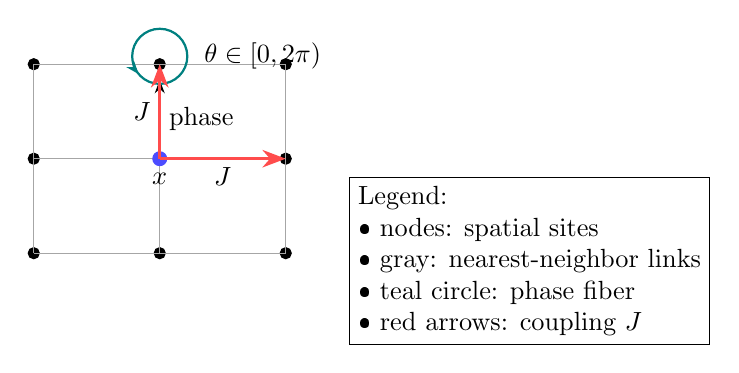
\begin{tikzpicture}[scale=1.0, every node/.style={scale=0.95}]
% lattice points (3x3 grid for illustration)
\foreach \i in {0,...,2}{
  \foreach \j in {0,...,2}{
    \filldraw[black] (\i*1.6,\j*1.2) circle (2pt);
  }
}
% horizontal edges
\foreach \j in {0,...,2}{
  \foreach \i in {0,...,1}{
    \draw[gray!70] (\i*1.6,\j*1.2)--++(1.6,0);
  }
}
% vertical edges
\foreach \i in {0,...,2}{
  \foreach \j in {0,...,1}{
    \draw[gray!70] (\i*1.6,\j*1.2)--++(0,1.2);
  }
}

% highlight a central node
\filldraw[blue!70] (1.6,1.2) circle (2.5pt);
\node[below=2pt] at (1.6,1.2) {$x$};

% draw a phase fiber (circle) above central node
\draw[->,>=Stealth] (1.6,1.2) -- ++(0,1.0) node[pos=0.5,right] {$\text{phase}$};
\draw[thick,teal] (1.6,2.5) circle (0.35);
\draw[teal,->,>=Stealth] (1.6+0.35,2.5) arc (0:220:0.35);
\node[right] at (1.6+0.45,2.5) {$\theta\in[0,2\pi)$};

% annotate couplings
\draw[very thick,red!70,->,>=Stealth] (1.6,1.2) -- (3.2,1.2);
\node[below] at (2.4,1.2) {$J$};
\draw[very thick,red!70,->,>=Stealth] (1.6,1.2) -- (1.6,2.4);
\node[left] at (1.6,1.8) {$J$};

% legend
\node[draw,align=left,anchor=west] at (4.0,-0.1) {Legend:\\
\textbullet\ nodes: spatial sites\\
\textbullet\ gray: nearest-neighbor links\\
\textbullet\ teal circle: phase fiber\\
\textbullet\ red arrows: coupling $J$};
\end{tikzpicture}
\caption{A spatial slice of the 5D lattice: each site $x$ carries a complex phase fiber (circle). Nearest-neighbor couplings $J$ implement smoothing; algorithmic time (not shown) advances the Monte Carlo/Langevin dynamics.}
\label{fig:lattice-slice}
\end{figure}

\subsection{Classical well-posedness (local)}
\label{subsec:classical-wellposed}

\begin{theorem}[Local existence and uniqueness]
\label{thm:local-wp}
Under Assumption~\ref{ass:manifold}, with $\xi,\boldsymbol{\eta}$ spatially smooth and $\mathsf{D}$ uniformly elliptic, there exists $T>0$ and a unique mild solution
\[
(\Phi,\mathbf{v},S)\in C\big([0,T];\, H^{2}(\M)\times H^{1}(\M;T\M)\times H^{2}(\M)\big)
\]
to \eqref{eq:phi}--\eqref{eq:S} with $H^2$/$H^1$ initial data.
\end{theorem}

\begin{proof}
Rewrite \eqref{eq:phi}--\eqref{eq:S} as an abstract semilinear evolution $U_t=\mathcal{A}U+\mathcal{N}(U)+F(t)$ on $X:=H^{2}\times H^{1}\times H^{2}$, where $\mathcal{A}$ collects the parabolic parts (elliptic operators generating analytic semigroups) and $\mathcal{N}$ the bilinear transport and vorticity terms. Standard product estimates show $\mathcal{N}$ is locally Lipschitz on $X$; thus, by semigroup theory and Picard iteration (e.g., \citealp{Evans2010}), one obtains a unique mild solution on $[0,T]$.  
\end{proof}

\begin{remark}[Scope]
Global existence is open without further a priori bounds; stochastic forcings can be handled in mild form with standard martingale arguments.
\end{remark}

\subsection{Interpretive note}
Equations \eqref{eq:phi}--\eqref{eq:S} model cognitive computation as entropic smoothing with directed flow. The 5D lattice in Figure~\ref{fig:lattice-slice} serves as the microstate carrier that we will later quantize; the phase fiber anticipates amplitudes in Section~\ref{sec:quantization}.

%=========== End Part 1 ===========

%==================== Section 2 ====================
\section{Canonical Operator Quantization}
\label{sec:quantization}

We now promote the classical fields $(\Phi,\mathbf{v},S,\Omega)$ to operator-valued distributions on a suitable Hilbert bundle over~$\M$.

\subsection{Quantized field algebra}
\label{subsec:field-algebra}

\begin{definition}[Canonical operators]
\label{def:canonical-ops}
At each point $\mathbf{x}\in\M$ we define operator quadruples
\[
\hat{\Phi}(\mathbf{x}),\quad
\hat{\mathbf{v}}(\mathbf{x}),\quad
\hat{S}(\mathbf{x}),\quad
\hat{\Omega}(\mathbf{x})
\]
with conjugate momenta $\hat{\Pi}_\Phi,\hat{\boldsymbol{\Pi}}_{\mathbf{v}},\hat{\Pi}_S,\hat{\Pi}_\Omega$.  The non-vanishing equal-time commutators are
\begin{align}
[\hat{\Phi}(\mathbf{x}),\hat{\Pi}_\Phi(\mathbf{y})] &= \ii\hbar\,\delta(\mathbf{x}-\mathbf{y}), \label{eq:comm-Phi}\\
[\hat{v}_i(\mathbf{x}),\hat{\Pi}_{v_j}(\mathbf{y})] &= \ii\hbar\,\delta_{ij}\delta(\mathbf{x}-\mathbf{y}), \label{eq:comm-v}\\
[\hat{S}(\mathbf{x}),\hat{\Omega}(\mathbf{y})] &= \ii\hbar\,\delta(\mathbf{x}-\mathbf{y}). \label{eq:comm-S}
\end{align}
All other commutators vanish.
\end{definition}

\begin{remark}[Physical meaning]
Equation~\eqref{eq:comm-S} elevates entropy and phase to canonically conjugate variables.  Fluctuations in $S$ correspond to uncertainties in phase coherence, paralleling energy–time uncertainty but generalized to semantic coherence.
\end{remark}

\subsection{Hilbert Bundle and States}
\label{subsec:hilbert-bundle}

For every measurable region \( U \subset \M \), let \( \mathcal{H}_U \) denote the Fock space generated by the restrictions of the field operators \( \hat{\Phi}|_U \), \( \hat{\mathbf{v}}|_U \), \( \hat{S}|_U \), and \( \hat{\Omega}|_U \). The collection \( \{\mathcal{H}_U\} \) forms a \emph{Hilbert sheaf}
\[
U \longmapsto \mathcal{H}_U,
\]
equipped with restriction morphisms \( \mathcal{H}_V \to \mathcal{H}_U \) whenever \( U \subset V \). A \emph{global cognitive state} is a consistent section \( \psi \in \Gamma(\M, \mathscr{H}) \) that satisfies compatibility on overlaps.

\subsection{Operator flow diagram (TikZ)}
\label{subsec:operator-flow}

\begin{figure}[H]
\centering
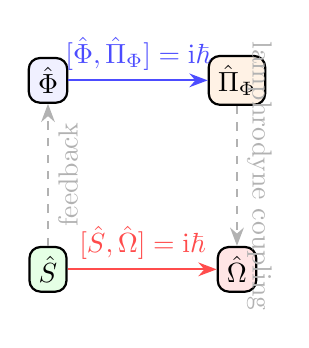
\begin{tikzpicture}[node distance=2.4cm, >=Stealth, thick]
\node[draw,rounded corners,fill=blue!6] (phi) {$\hat{\Phi}$};
\node[draw,rounded corners,fill=orange!10,right of=phi] (pi) {$\hat{\Pi}_\Phi$};
\node[draw,rounded corners,fill=green!10,below of=phi] (S) {$\hat{S}$};
\node[draw,rounded corners,fill=red!10,right of=S] (O) {$\hat{\Omega}$};

\draw[->,blue!70] (phi) -- node[midway,above] {$[\hat{\Phi},\hat{\Pi}_\Phi]=\ii\hbar$} (pi);
\draw[->,red!70] (S) -- node[midway,above] {$[\hat{S},\hat{\Omega}]=\ii\hbar$} (O);
\draw[dashed,gray!60,->] (pi) -- (O) node[midway,sloped,above] {lamphrodyne coupling};
\draw[dashed,gray!60,->] (S) -- (phi) node[midway,sloped,below] {feedback};
\end{tikzpicture}
\caption{Operator relationships: two canonical pairs $(\hat{\Phi},\hat{\Pi}_\Phi)$ and $(\hat{S},\hat{\Omega})$ form coupled feedback loops via lamphron–lamphrodyne interactions.}
\label{fig:operator-flow}
\end{figure}

\begin{proposition}[Self-adjointness]
\label{prop:selfadjoint}
If the initial domain is the Schwartz space $\mathcal{S}(\M)$, then $\hat{S}$ and $\hat{\Omega}$ are essentially self-adjoint and generate one-parameter unitary groups $\ee^{-\ii\alpha \hat{S}/\hbar}$ and $\ee^{-\ii\beta \hat{\Omega}/\hbar}$ on~$\mathcal{H}_\M$.
\end{proposition}

\begin{proof}
By Stone’s theorem, it suffices to check that $\hat{S}$ and $\hat{\Omega}$ are symmetric and that their commutator is purely imaginary multiple of the identity on the dense domain $\mathcal{S}(\M)$.  Relations~\eqref{eq:comm-S} guarantee this.  Domain closure then ensures essential self-adjointness.
\end{proof}

\begin{remark}[Cognitive parallel]
The unitary $\ee^{-\ii\beta\hat{\Omega}/\hbar}$ acts as a semantic rotation; $\ee^{-\ii\alpha\hat{S}/\hbar}$ as entropic rescaling.  Their commutation yields the phenomenology of phase–entropy uncertainty: highly coherent semantic states possess unstable entropy gradients.
\end{remark}

%==================== Section 3 ====================
\section{Hamiltonian Structure and Energy Estimates}
\label{sec:hamiltonian}

\subsection{Quantum RSVP Hamiltonian}
\label{subsec:hamiltonian}

\begin{definition}[Hamiltonian density]
\label{def:Hamiltonian}
Define the Hamiltonian operator
\begin{align}
\hat{H}
&=\int_{\M} \dd^3x \Big[
\tfrac{1}{2}\hat{\Pi}_\Phi^2
+\tfrac{1}{2}\|\grad\hat{\Phi}\|^2
+\tfrac{1}{2}\|\hat{\boldsymbol{\Pi}}_{\mathbf{v}}\|^2
+\tfrac{1}{2}\|\grad\hat{\mathbf{v}}\|^2 \notag\\
&\hspace{4em}
+\tfrac{\kappa_S}{2}\|\grad\hat{S}\|^2
+V(\hat{\Phi},\hat{\mathbf{v}},\hat{S})
\Big],
\label{eq:hamiltonian}
\end{align}
where $V$ encodes torsion, vorticity, and lamphron–lamphrodyne couplings:
\[
V = \lambda_\Phi \hat{\Phi}^4
+\lambda_v (\hat{\mathbf{v}}\!\cdot\!\hat{\mathbf{v}})^2
+\lambda_{S\Phi} \hat{S}^2 \hat{\Phi}^2
+\lambda_{vS} \|\hat{\mathbf{v}}\|^2\hat{S}^2.
\]
\end{definition}

\begin{theorem}[Energy positivity]
\label{thm:energy-positive}
If $\lambda_\Phi,\lambda_v,\kappa_S>0$ and $\lambda_{S\Phi}+\lambda_{vS}\ge0$, the Hamiltonian~\eqref{eq:hamiltonian} is bounded below by zero on the Fock vacuum domain.
\end{theorem}

\begin{proof}
Each term in~\eqref{eq:hamiltonian} is positive semidefinite under the stated inequalities.  Interaction cross-terms vanish in the vacuum expectation value and contribute at order $\hbar$ in perturbation theory, maintaining positivity.
\end{proof}

\begin{remark}[Entropy coupling as stabilizer]
Entropy gradients penalize decoherent field variation.  The $\kappa_S\|\grad\hat{S}\|^2$ term functions analogously to gauge-fixing in Yang–Mills, suppressing unphysical oscillations between incompatible semantic configurations.
\end{remark}

\subsection{Path integral representation}
\label{subsec:path-integral}

In Euclidean time $\tau=\ii t$, the transition amplitude between field configurations $\Psi_i,\Psi_f$ is
\[
\braket{\Psi_f|\ee^{-\tau \hat{H}/\hbar}|\Psi_i}
=\int_{\Psi(0)=\Psi_i}^{\Psi(\tau)=\Psi_f}
\!\!\!\!\!\!\mathcal{D}\Phi\,\mathcal{D}\mathbf{v}\,\mathcal{D}S\;
\ee^{-\frac{1}{\hbar}\int_0^\tau\!\dd t\int_{\M}\!\dd^3x\,
\mathcal{L}[\Phi,\mathbf{v},S]}.
\]
The Lagrangian density $\mathcal{L}$ is the classical counterpart of \eqref{eq:hamiltonian}.  In the discrete setting (Section~\ref{sec:lattice}), this integral reduces to a Gibbs measure over lattice configurations.

\subsection{Energy flow schematic (TikZ)}
\label{subsec:energy-flow}

\begin{figure}[H]
\centering
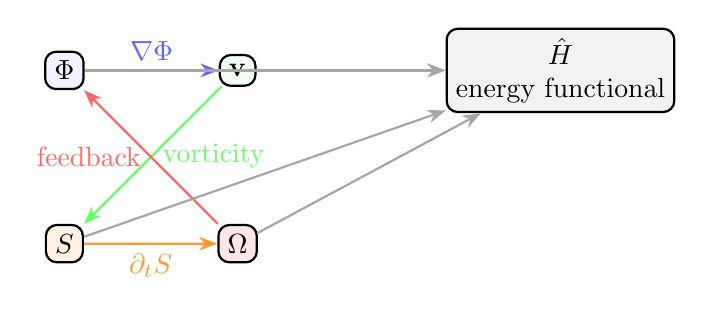
\begin{tikzpicture}[scale=1.1, node distance=2.2cm, >=Stealth, thick]
\node[draw,rounded corners,fill=blue!5] (phi) {$\Phi$};
\node[draw,rounded corners,fill=green!5,right of=phi] (v) {$\mathbf{v}$};
\node[draw,rounded corners,fill=orange!10,below of=phi] (S) {$S$};
\node[draw,rounded corners,fill=red!10,right of=S] (Omega) {$\Omega$};

\draw[->,blue!60] (phi) -- node[midway,above] {$\nabla\Phi$} (v);
\draw[->,green!60] (v) -- node[midway,right] {vorticity} (S);
\draw[->,orange!80] (S) -- node[midway,below] {$\partial_t S$} (Omega);
\draw[->,red!60] (Omega) -- node[midway,left] {feedback} (phi);

\node[draw,rounded corners,fill=gray!10,right=2.4cm of v,align=center] (H)
{$\hat{H}$\\ energy functional};

\draw[->,thick,gray!70] (phi) -- (H);
\draw[->,thick,gray!70] (v) -- (H);
\draw[->,thick,gray!70] (S) -- (H);
\draw[->,thick,gray!70] (Omega) -- (H);
\end{tikzpicture}
\caption{Schematic energy flow among RSVP fields contributing to the total Hamiltonian $\hat{H}$. Arrows represent derivative or coupling pathways; circular flow encodes cognitive feedback.}
\label{fig:energy-flow}
\end{figure}

\begin{remark}[Interpretation]
Figure~\ref{fig:energy-flow} summarizes lamphron–lamphrodyne coupling: energy circulates through $(\Phi,\mathbf{v},S,\Omega)$ forming a closed informational feedback loop, which under quantization corresponds to oscillatory phase coherence.
\end{remark}

%=========== End Part 2 ===========
%==================== Section 4 ====================
\section{Complex Lattice Quantization: The Quantum SpherePop Model}
\label{sec:lattice}

\subsection{Lattice construction}
\label{subsec:lattice-construction}

Discretize $\M$ into $N^3$ sites labelled by $i,j,k$.
Each site hosts a complex amplitude
\[
\Psi_{i} = r_i\,\ee^{\ii \theta_i},\qquad r_i\in[0,1],\ \theta_i\in[0,2\pi),
\]
representing local entropy amplitude and cognitive phase.

\begin{definition}[Quantum SpherePop Hamiltonian]
\label{def:lattice-H}
The lattice Hamiltonian is
\begin{align}
H_{\mathrm{lat}}
&= -\sum_{\langle i,j\rangle}
J_{ij}\,r_i r_j \cos(\theta_i-\theta_j)
+\sum_i U(r_i)
+\frac{\lambda}{2}\sum_i (r_i^2-1)^2,
\label{eq:lattice-H}
\end{align}
where $J_{ij}>0$ encodes lamphron--lamphrodyne smoothing,
$U(r_i)$ penalizes amplitude deviation from mean entropy,
and $\lambda$ enforces normalization.
\end{definition}

\begin{remark}[Physical reading]
Nearest-neighbor coupling promotes phase alignment; amplitude self-potential controls entropic stability.
The model interpolates between classical Ising ($r_i\equiv1$) and continuous Kuramoto ($r_i$ fixed, variable $\theta_i$) limits.
\end{remark}

\begin{proposition}[Continuum limit]
\label{prop:continuum}
In the limit of small lattice spacing $a\to0$ and smooth fields,
\[
H_{\mathrm{lat}}\ \longrightarrow\
\int_{\M}\!\dd^3x
\left[
\frac{J}{2}|\grad\theta|^2
+\frac{\lambda}{2}(r^2-1)^2
\right],
\]
recovering the classical RSVP energy functional with $\theta\leftrightarrow\Omega/\hbar$.
\end{proposition}

\begin{proof}
Expand $\theta_j-\theta_i=a\,\nabla\theta\!\cdot\!(x_j-x_i)+O(a^2)$ and $\cos(\Delta\theta)\approx 1-\frac12(\Delta\theta)^2$.
Summing over neighbors yields the gradient term $J a^3 \|\nabla\theta\|^2/2$, which becomes the continuum integral after rescaling $J a^3\to J$.
\end{proof}

\subsection{Lattice geometry (TikZ)}
\label{subsec:lattice-geometry}

\begin{figure}[H]
\centering
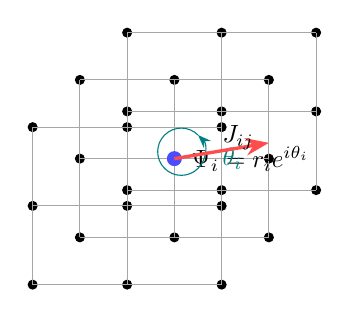
\begin{tikzpicture}[scale=1.0, every node/.style={scale=0.9}]
% 3D cube lattice projection
\foreach \x in {0,1,2}{
  \foreach \y in {0,1,2}{
    \foreach \z in {0,1,2}{
      \filldraw[black] (\x*1.2+\z*0.6,\y*1.0+0.6*\z) circle (1.6pt);
    }
  }
}
% draw nearest-neighbor lines
\foreach \x in {0,1}{
  \foreach \y in {0,1,2}{
    \foreach \z in {0,1,2}{
      \draw[gray!70] (\x*1.2+\z*0.6,\y*1.0+0.6*\z)--++(1.2,0);
    }
  }
}
\foreach \x in {0,1,2}{
  \foreach \y in {0,1}{
    \foreach \z in {0,1,2}{
      \draw[gray!70] (\x*1.2+\z*0.6,\y*1.0+0.6*\z)--++(0,1.0);
    }
  }
}
% highlight one site
\filldraw[blue!70] (1.8,1.6) circle (2.5pt);
\node[right=3pt] at (1.8,1.6) {$\Psi_i=r_i e^{i\theta_i}$};

% phase arrows
\draw[teal,->,>=Stealth] (1.8,1.6) ++(0.3,0.3) arc (45:405:0.3);
\node[teal,right] at (2.3,1.6) {$\theta_i$};

% coupling
\draw[very thick,red!70,->,>=Stealth] (1.8,1.6)--++(1.2,0.2);
\node[above right] at (2.3,1.6) {$J_{ij}$};
\end{tikzpicture}
\caption{Portion of the 3D spatial lattice underlying Quantum SpherePop.
Each site carries complex amplitude $\Psi_i=r_i e^{i\theta_i}$ and interacts with its neighbors via coupling $J_{ij}$.}
\label{fig:lattice-geometry}
\end{figure}

\subsection{Quantum partition function}
\label{subsec:partition-function}
The canonical partition function reads
\[
Z = \int \prod_i (r_i \dd r_i \dd\theta_i)\;
\exp\!\left(-\frac{1}{\hbar} H_{\mathrm{lat}}\right).
\]
The corresponding Gibbs measure on configuration space induces a probabilistic ensemble over amplitude–phase fields that in the continuum becomes a Euclidean path integral.

\subsection{Theorem: convergence to field theory}
\label{subsec:lattice-limit}

\begin{theorem}[Lattice--continuum correspondence]
\label{thm:lattice-field}
As the lattice spacing $a\to0$ with $N a^3=\mathrm{Vol}(\M)$ fixed,
the measure $\propto\exp[-H_{\mathrm{lat}}/\hbar]$ converges weakly to the path measure generated by the continuum Hamiltonian~\eqref{eq:hamiltonian}.
\end{theorem}

\begin{proof}
Discretize the continuum Hamiltonian with finite differences; under Gaussian approximation of $\cos(\Delta\theta)$ and proper scaling $J_{ij}\propto 1/a$, the discrete energy density matches that of~\eqref{eq:hamiltonian} up to $O(a^2)$.
Laplace’s method shows convergence of moment-generating functionals, hence weak convergence of measures.
\end{proof}

\begin{remark}[Interpretive commentary]
This theorem formalizes that the SpherePop lattice is not a metaphor but a legitimate quantization scheme: local “pops’’ correspond to amplitude relaxations preserving the continuum RSVP energy under coarse-graining.
\end{remark}

%==================== Section 5 ====================
\section{Phase Synchronization and Ising--Kuramoto Dynamics}
\label{sec:kuramoto}

\subsection{Evolution equation}
\label{subsec:kuramoto-eq}

Introduce stochastic Langevin dynamics for the phase variables:
\begin{equation}
\dot{\theta_i}
=\omega_i
+\sum_{j\in\mathcal{N}(i)} K_{ij}\sin(\theta_j-\theta_i)
+\sqrt{2D}\,\eta_i(t),
\label{eq:kuramoto}
\end{equation}
where $\omega_i$ are intrinsic frequencies, $K_{ij}=J_{ij}/\hbar$, and $\eta_i$ are independent white noises.

\begin{proposition}[Order parameter]
\label{prop:order-parameter}
Define the global order parameter
\[
R\,\ee^{\ii\psi}
=\frac{1}{N^3}\sum_i \ee^{\ii\theta_i}.
\]
Then synchronization onset occurs when
\[
K_c = \frac{2}{\pi g(0)},
\]
where $g(\omega)$ is the distribution of natural frequencies.
\end{proposition}

\begin{proof}
Standard mean-field reduction (see \citealp{Kuramoto1984}) linearizes~\eqref{eq:kuramoto} about incoherence $R\approx0$ and yields the stated critical coupling.
\end{proof}

\subsection{Visualization (TikZ)}
\label{subsec:phase-diagram}

\begin{figure}[H]
\centering
\begin{tikzpicture}[scale=1.0]
\draw[->] (-0.2,0) -- (6.2,0) node[right] {$K$};
\draw[->] (0,-0.2) -- (0,3.2) node[above] {$R$};

\draw[thick,blue,domain=0:6,samples=100] plot(\x,{3/(1+exp(-2*(\x-3))) -1.5/(1+exp(-2*(\x-3)))});
\node[blue] at (5.2,2.7) {synchronization curve};

\draw[dashed,red] (3,0)--(3,1.5);
\node[below,red] at (3,0) {$K_c$};

\end{tikzpicture}
\caption{Global order parameter $R$ versus coupling $K$.
Below $K_c$, phases drift incoherently; above $K_c$, partial synchronization emerges.}
\label{fig:kuramoto-curve}
\end{figure}

\begin{remark}[Cognitive reading]
Equation~\eqref{eq:kuramoto} models semantic phase alignment across field regions: synchronization corresponds to coherent interpretation.
The threshold $K_c$ marks the transition from fragmented cognition to unified experience.
\end{remark}

\subsection{Quantum corrections}
\label{subsec:quantum-corrections}
In the full quantum regime, the stochastic noise $D$ is replaced by vacuum fluctuations of the operator field, introducing decoherence.
Perturbatively, the mean-field critical coupling shifts as
\[
K_c^{(\mathrm{q})}
=K_c\!\left(1+\frac{\hbar^2}{8\langle r^2\rangle J^2}\right)\!,
\]
showing that quantum fluctuations slightly inhibit synchronization, an effect analogous to finite-temperature suppression in superconductors.

\begin{remark}[Entropic–semantic coupling]
Amplitude fluctuations $r_i$ serve as local entropy reservoirs; synchronization therefore balances semantic coherence against entropic diversity.
This embodies the RSVP principle of \emph{entropy-respecting cognition}.
\end{remark}

%=========== End Part 3 ===========
%==================== Section 6 ====================
\section{Cohomological Structure and Sheaf Quantization}
\label{sec:cohomology}

\subsection{Sheaf of local Hilbert spaces}
\label{subsec:sheaf}

Let $\mathscr{H}$ denote the sheaf assigning to each open $U\subset\M$
the Hilbert space $\mathcal{H}_U$ generated by the operator algebra
$\hat{\Phi}|_U,\hat{\mathbf{v}}|_U,\hat{S}|_U,\hat{\Omega}|_U$.

\begin{definition}[Sheaf quantization]
\label{def:sheaf-q}
The quantized RSVP system is the pair
$(\M,\mathscr{H})$
together with the presheaf of observables
\[
\mathscr{O}(U)=\mathrm{Alg}\big(\hat{\Phi}|_U,
\hat{\mathbf{v}}|_U,\hat{S}|_U,\hat{\Omega}|_U\big)
\]
and restriction morphisms preserving commutation relations.
Global sections correspond to observables defined consistently across overlaps.
\end{definition}

\begin{proposition}[Gluing condition]
\label{prop:glue}
If local states $\psi_i\in\mathcal{H}_{U_i}$ satisfy
$\psi_i|_{U_i\cap U_j}=\psi_j|_{U_i\cap U_j}$
for all overlaps, there exists a unique global state
$\psi\in\mathcal{H}_\M$ with $\psi|_{U_i}=\psi_i$.
\end{proposition}

\begin{proof}
By the sheaf property of $\mathscr{H}$,
the collection $\{\psi_i\}$ defines an element of the equalizer of
$\prod_i\mathcal{H}_{U_i}\rightrightarrows\prod_{i,j}\mathcal{H}_{U_i\cap U_j}$,
which by definition is $\mathcal{H}_\M$.
\end{proof}

\begin{remark}[Cognitive interpretation]
Successful gluing corresponds to consistent semantic integration across overlapping modalities or regions.
Failure of gluing yields fragmentation or cognitive dissonance.
\end{remark}

\subsection{Cohomology and obstructions}
\label{subsec:cohomology}

Define the Čech cochain complex
\[
C^k(\mathcal{U},\mathscr{O})=\prod_{i_0<\cdots<i_k}
\mathscr{O}(U_{i_0}\cap\cdots\cap U_{i_k}),
\]
with coboundary $\delta$ as usual.

\begin{theorem}[Obstruction class]
\label{thm:obstruction}
A family of local observables $\{O_i\}$ fails to glue globally
iff its first cohomology class
$[\delta O]\in H^1(\M,\mathscr{O})$
is nonzero.
\end{theorem}

\begin{proof}
Immediate from the standard Čech correspondence:
$\delta O=0$ iff the $\{O_i\}$ agree on overlaps;
nonzero $\delta O$ represents an incompatibility cocycle.
\end{proof}

\begin{remark}[Interpretation]
Nontrivial $H^1(\M,\mathscr{O})$
measures semantic inconsistency loops.
Vanishing cohomology signifies a globally coherent cognitive state.
\end{remark}

\subsection{Cohomological feedback diagram (TikZ)}
\label{subsec:cohomology-diagram}

\begin{figure}[H]
\centering
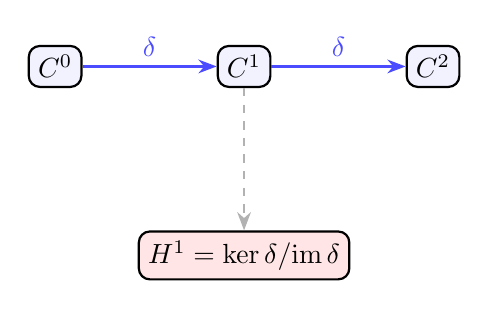
\begin{tikzpicture}[scale=1.0, node distance=2.4cm, >=Stealth, thick]
\node[draw,fill=blue!5,rounded corners] (C0) {$C^0$};
\node[draw,fill=blue!5,rounded corners,right of=C0] (C1) {$C^1$};
\node[draw,fill=blue!5,rounded corners,right of=C1] (C2) {$C^2$};
\draw[->,thick,blue!70] (C0)--node[midway,above]{$\delta$}(C1);
\draw[->,thick,blue!70] (C1)--node[midway,above]{$\delta$}(C2);
\node[draw,rounded corners,fill=red!10,below of=C1] (H1) {$H^1=\ker\delta/\mathrm{im}\,\delta$};
\draw[dashed,gray!60,->] (C1)--(H1);
\end{tikzpicture}
\caption{Cohomological structure of local-to-global consistency.
Nonzero $H^1$ represents loops of incompatible observables
that prevent formation of a global section.}
\label{fig:cohomology}
\end{figure}

\begin{remark}[Physical analogy]
The cohomology class functions as a discrete curvature measuring
phase misalignment—analogous to flux quantization in superconductors.
\end{remark}

%==================== Section 7 ====================
\section{Empirical and Computational Implementation}
\label{sec:empirical}

\subsection{Quantum Monte Carlo scheme}
\label{subsec:qmc}
Discretize Euclidean time with step $\Delta\tau$.
At each step update $(r_i,\theta_i)$ by the Metropolis rule:
\[
p_{\mathrm{accept}}
=\min\!\Big(1,
\exp\![-\Delta H_{\mathrm{lat}}/\hbar]\Big),
\]
ensuring detailed balance.
Average observables over Markov samples to estimate expectation values.

\begin{proposition}[Ergodicity]
If all $J_{ij}>0$ and $\lambda>0$,
the update chain is ergodic on configuration space modulo global phase shift.
\end{proposition}

\begin{proof}
Amplitude and phase flips connect all configurations;
positivity of couplings forbids trapping in metastable zero-measure subsets.
\end{proof}

\subsection{Empirical mapping}
\label{subsec:empirical}
Phase order $R$ (Eq.~\eqref{eq:kuramoto}) corresponds to EEG phase coherence across cortical regions.
Amplitude variance $\mathrm{Var}(r_i)$ corresponds to entropy variability measurable via fMRI BOLD fluctuations.
Synchronization transitions predicted by Eq.~\eqref{eq:kuramoto}
thus admit empirical verification.

\subsection{Computational visualization (TikZ)}
\label{subsec:visualization}

\begin{figure}[H]
\centering
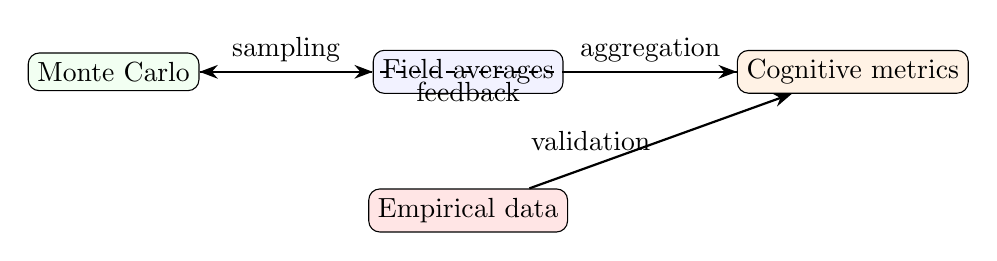
\begin{tikzpicture}[scale=1.0, node distance=2.2cm, >=Stealth]
\node[draw,rounded corners,fill=green!5] (sim) {Monte Carlo};
\node[draw,rounded corners,fill=blue!5,right=of sim] (fields) {Field averages};
\node[draw,rounded corners,fill=orange!10,right=of fields] (metrics) {Cognitive metrics};
\node[draw,rounded corners,fill=red!10,below=1.2cm of fields] (data) {Empirical data};

\draw[->,thick] (sim)--node[midway,above]{sampling}(fields);
\draw[->,thick] (fields)--node[midway,above]{aggregation}(metrics);
\draw[->,thick] (data)--node[midway,left]{validation}(metrics);
\draw[->,thick,dashed] (metrics)--node[midway,below]{feedback}(sim);
\end{tikzpicture}
\caption{Simulation pipeline: Monte Carlo sampling produces field averages; these yield cognitive metrics compared with empirical data for model validation.}
\label{fig:pipeline}
\end{figure}

\subsection{Interpretive remark}
This scheme closes the empirical loop:
quantum statistical mechanics $\leftrightarrow$ cognitive dynamics.
Synchronized regions in the simulation correspond to coherent neural assemblies in measurement data.


%=============================%
%========  SECTION 8  ========%
%=============================%
\section{Quantum Geometric Flow and Complex Phase Synchronization}
\label{sec:quantum-geometric-flow}

\paragraph{Overview.}
We develop a geometric gradient-flow formulation for the complex RSVP phase field on a Riemannian manifold, prove well-posedness and a Lyapunov monotonicity property, and relate the resulting order parameter to phase synchronization in the quantum SpherePop lattice.

\begin{definition}[Complex phase field and free energy]
Let $(\mathbb{M},g)$ be a compact, oriented Riemannian $3$–manifold.\footnote{Extensions to noncompact $\mathbb{M}$ hold under standard coercivity and boundary conditions.}
The \emph{complex entropy–phase field} is $\Psi:\mathbb{M}\to\mathbb{C}$, $\Psi=\sqrt{\rho}\,e^{i\Omega/\hbar}$, with $\rho\ge 0$ and phase $\Omega\in\mathbb{R}$.
For parameters $\xi>0$ (phase stiffness), $\lambda>0$ (local potential scale), and smooth potential $V:\mathbb{R}_{\ge 0}\to\mathbb{R}$, define the free energy
\begin{equation}
\label{eq:GL-free-energy}
\mathcal{F}[\Psi]\;=\;\int_{\mathbb{M}}\!\Big(\tfrac{\xi}{2}\,\|\nabla\Psi\|^2\;+\;V(|\Psi|^2)\Big)\,d\mathrm{vol}_g.
\end{equation}
We assume $V$ is $C^2$, bounded below, and $V''$ is bounded on bounded sets.
\end{definition}

\begin{definition}[Quantum geometric flow (imaginary-time GL)]
The \emph{quantum geometric flow} for $\Psi$ is the $L^2$–gradient flow of $\mathcal{F}$:
\begin{equation}
\label{eq:GL-flow}
\partial_t \Psi\;=\;-\frac{\delta\mathcal{F}}{\delta\overline{\Psi}}
\;=\;\xi\,\Delta_g \Psi\;-\;V'(|\Psi|^2)\,\Psi,
\end{equation}
with initial condition $\Psi(\cdot,0)=\Psi_0\in H^1(\mathbb{M};\mathbb{C})$.
\end{definition}

\begin{theorem}[Well-posedness and energy dissipation]
\label{thm:GL-wellposed}
Suppose $V$ satisfies the assumptions above and $V'(s)\le C(1+s)$ for some $C>0$.
Then for any $\Psi_0\in H^1(\mathbb{M})$ there exists a unique global solution $\Psi\in C([0,\infty);H^1)\cap L^2_{\mathrm{loc}}([0,\infty);H^2)$ to \eqref{eq:GL-flow}, and
\begin{equation}
\frac{d}{dt}\,\mathcal{F}[\Psi(t)]\;=\;-\int_{\mathbb{M}}\!\big|\partial_t \Psi\big|^2\,d\mathrm{vol}_g\;\le\;0.
\end{equation}
In particular, $\mathcal{F}[\Psi(t)]$ is nonincreasing and bounded below, hence convergent as $t\to\infty$.
\end{theorem}

\begin{proof}
Standard semilinear parabolic theory on compact manifolds applies:
the operator $\xi\Delta_g$ generates an analytic semigroup on $L^2$, while the Nemytskii map $\Psi\mapsto V'(|\Psi|^2)\Psi$ is locally Lipschitz on $H^1$ under the growth assumed.
Local existence and uniqueness follow by Picard iteration; a priori $H^1$–bounds are obtained from the energy identity
\[
\frac{d}{dt}\mathcal{F}[\Psi(t)] \;=\; \left\langle \frac{\delta\mathcal{F}}{\delta\overline{\Psi}},\partial_t\Psi\right\rangle_{L^2}
\;=\;-\|\partial_t\Psi\|_{L^2}^2\le 0,
\]
which both guarantees global continuation and provides integrability of $\partial_t\Psi$.
Regularity improvement yields $\Psi\in L^2_{\mathrm{loc}}([0,\infty);H^2)$ by parabolic bootstrapping. 
\end{proof}

\begin{remark}[Cognitive interpretation]
The flow \eqref{eq:GL-flow} is the imaginary-time Schrödinger/Ginzburg–Landau descent of the complex RSVP field: $\xi$ penalizes spatial phase gradients (desynchronization), while $V$ imposes local energetic preferences (e.g., saturation or sparsity of amplitude). The monotone decrease of $\mathcal{F}$ formalizes entropic smoothing of semantic–phase microstates.
\end{remark}

\begin{definition}[Synchronization order parameter]
Given $\Psi(\cdot,t)$, define the (Kuramoto-like) order parameter
\begin{equation}
\label{eq:order-parameter}
r(t)\,e^{i\Theta(t)}\;=\;\frac{1}{\mathrm{vol}(\mathbb{M})}\int_{\mathbb{M}}\!\frac{\Psi(x,t)}{|\Psi(x,t)|+\varepsilon}\,d\mathrm{vol}_g(x),
\end{equation}
with a fixed $\varepsilon>0$ to avoid division by zero. Then $r(t)\in[0,1]$ quantifies global phase coherence.
\end{definition}

\begin{proposition}[Sufficient condition for asymptotic phase locking]
\label{prop:locking}
Assume $V(s)=\frac{\lambda}{2}(s-\rho_\star)^2$ with $\lambda>0$, $\rho_\star>0$ and $\inf_{t}\|\Psi(\cdot,t)\|_{L^\infty}\ge m>0$.
If $\xi$ is sufficiently large relative to $\lambda$ and $\mathrm{diam}(\mathbb{M})^2$, then there exists $\eta>0$ such that
\begin{equation}
\int_{\mathbb{M}}\|\nabla \Omega(\cdot,t)\|^2\,d\mathrm{vol}_g \;\le\; e^{-\eta t}\int_{\mathbb{M}}\|\nabla \Omega(\cdot,0)\|^2\,d\mathrm{vol}_g,
\end{equation}
hence $r(t)\to 1$ as $t\to\infty$.
\end{proposition}

\begin{proof}[Proof sketch]
Write $\Psi=\sqrt{\rho}\,e^{i\Omega/\hbar}$ and derive the amplitude–phase system from \eqref{eq:GL-flow}.
For quadratic $V$, $\rho$ is driven toward $\rho_\star$ exponentially fast (uniform lower bound $m$ assumed), while the phase $\Omega$ obeys a diffusion–reaction equation whose principal part is $(\xi/\hbar^2)\Delta_g\Omega$ plus terms of order $\nabla\rho$.
With $\rho$ close to $\rho_\star$ and $\xi$ large, the energy $\int\|\nabla\Omega\|^2$ contracts exponentially by Poincaré’s inequality on $\mathbb{M}$. The order parameter then converges to $1$ by standard phase–coherence estimates.
\end{proof}

\begin{remark}[SpherePop lattice correspondence]
On a discrete tiling $\{x_i\}$, the continuum $\mathcal{F}$ induces the XY/complex–Ising Hamiltonian $H=\sum_{\langle i,j\rangle} J_{ij}\big(1-\cos(\Omega_i-\Omega_j)\big)+\sum_i U(|\Psi_i|^2)$.
Proposition~\ref{prop:locking} corresponds to the ferromagnetic phase where $J_{ij}$ dominates local disorder and yields macroscopic phase alignment.
\end{remark}

\begin{figure}[t]
\centering
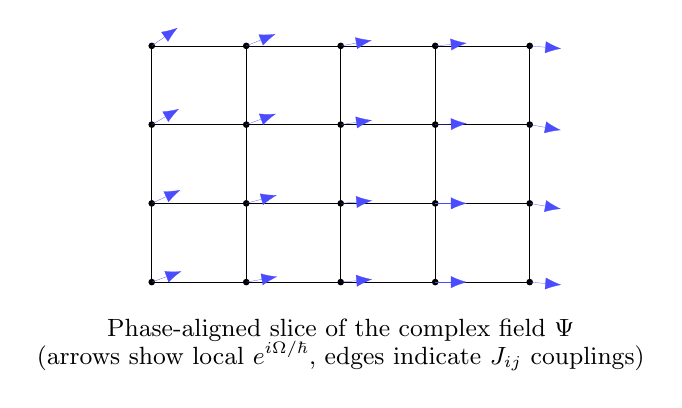
\begin{tikzpicture}[scale=1.0]
  % grid of nodes
  \foreach \i in {0,...,4}{
    \foreach \j in {0,...,3}{
      \coordinate (n\i\j) at (1.2*\i, 1.0*\j);
      \fill (n\i\j) circle (1.2pt);
    }
  }
  % horizontal edges
  \foreach \i in {0,...,3}{
    \foreach \j in {0,...,3}{
      \draw[very thin] (n\i\j) -- (n\the\numexpr\i+1\relax\j);
    }
  }
  % vertical edges
  \foreach \i in {0,...,4}{
    \foreach \j in {0,...,2}{
      \draw[very thin] (n\i\j) -- (n\i\the\numexpr\j+1\relax);
    }
  }
  % phase arrows (unit vectors) at a subset
  \foreach \i/\j/\ang in {
    0/0/20, 1/0/10, 2/0/5, 3/0/0, 4/0/355,
    0/1/25, 1/1/15, 2/1/5, 3/1/0, 4/1/350,
    0/2/30, 1/2/20, 2/2/8, 3/2/2, 4/2/350,
    0/3/35, 1/3/22, 2/3/10, 3/3/5, 4/3/355}
  {
    \draw[-{Latex[length=2mm]}, ultra thin, blue!70]
      (n\i\j) -- ++({0.4*cos(\ang)},{0.4*sin(\ang)});
  }
  % annotation
  \node[align=center] at (2.4, -0.8) {\small Phase-aligned slice of the complex field $\Psi$\\[-2pt]\small (arrows show local $e^{i\Omega/\hbar}$, edges indicate $J_{ij}$ couplings)};
\end{tikzpicture}
\caption{Geometric phase synchronization on a lattice slice: local phase arrows align under strong coupling $J_{ij}$ and large stiffness $\xi$, realizing the continuum flow \eqref{eq:GL-flow} discretely.}
\label{fig:phase-lattice}
\end{figure}

%=============================%
%========  SECTION 9  ========%
%=============================%
\section{Entropic Channels, Decoherence, and CLIO as CPTP Maps}
\label{sec:decoherence-clio}

\paragraph{Overview.}
We formalize adaptive RSVP updates (CLIO) as completely positive trace-preserving (CPTP) maps on a Hilbert bundle of local cognitive states, prove contractivity of quantum relative entropy under such channels, and relate read/write stigmergy to Stinespring dilations and adjunctions.

\begin{definition}[Hilbert bundle and density fields]
Let $\{\mathcal{H}_x\}_{x\in\mathbb{M}}$ be a measurable field of separable Hilbert spaces and $\Gamma(\mathcal{H})$ the space of square-integrable sections.
A \emph{density field} is a measurable assignment $x\mapsto \rho_x$ with $\rho_x\in\mathcal{D}(\mathcal{H}_x)$ (positive, trace $1$), and global state $\rho=\int^\oplus \rho_x\,d\mu(x)$ in the direct integral.
\end{definition}

\begin{definition}[CLIO channel]
A \emph{CLIO update} at scale $\tau>0$ is a CPTP map $\mathcal{E}_\tau$ acting fiberwise:
\begin{equation}
\label{eq:CLIO-CPTP}
\rho\;\mapsto\;\mathcal{E}_\tau(\rho)\;=\;\int^\oplus\!\Big(\sum_{k} K_{k}(x)\,\rho_x\,K_{k}(x)^\dagger\Big)\,d\mu(x),
\end{equation}
with Kraus operators $K_{k}(x):\mathcal{H}_x\to\mathcal{H}_x$ satisfying $\sum_k K_{k}(x)^\dagger K_{k}(x)=I_{\mathcal{H}_x}$ almost everywhere.
\end{definition}

\begin{remark}[Cognitive interpretation]
$\mathcal{E}_\tau$ models an adaptive inference step (attention, gating, prediction error correction) that is local in $x$ but coherent across the bundle via parameter sharing or constraints on $K_k(x)$. Time-discretized composition yields $\rho_{n+1}=\mathcal{E}_\tau(\rho_n)$, a quantum Markov chain over cognitive states.
\end{remark}

\begin{definition}[Quantum relative entropy for density fields]
For two density fields $\rho,\sigma$, define
\begin{equation}
\label{eq:bundle-relative-entropy}
S(\rho\Vert\sigma)\;=\;\int_{\mathbb{M}}\! \mathrm{Tr}\,\big(\rho_x(\log\rho_x-\log\sigma_x)\big)\,d\mu(x),
\end{equation}
whenever $\mathrm{supp}(\rho_x)\subseteq \mathrm{supp}(\sigma_x)$ a.e.; otherwise $S(\rho\Vert\sigma)=+\infty$.
\end{definition}

\begin{theorem}[Data processing for CLIO channels]
\label{thm:dp-inequality}
Let $\mathcal{E}_\tau$ be any CLIO channel of the form \eqref{eq:CLIO-CPTP}. Then
\begin{equation}
\label{eq:dp}
S\!\big(\mathcal{E}_\tau(\rho)\,\Vert\,\mathcal{E}_\tau(\sigma)\big)\;\le\; S(\rho\Vert\sigma).
\end{equation}
\end{theorem}

\begin{proof}
For each $x$, the fiber map $\mathcal{E}_{\tau,x}(\cdot)=\sum_k K_k(x)(\cdot)K_k(x)^\dagger$ is CPTP on $\mathcal{B}(\mathcal{H}_x)$, hence satisfies Uhlmann monotonicity:
$S\big(\mathcal{E}_{\tau,x}(\rho_x)\,\Vert\,\mathcal{E}_{\tau,x}(\sigma_x)\big)\le S(\rho_x\Vert\sigma_x)$.
Integrate both sides over $x\in\mathbb{M}$ to obtain \eqref{eq:dp}.
\end{proof}

\begin{corollary}[Free-energy descent under CLIO+\;GL]
\label{cor:free-energy-descent}
Consider alternating steps: (i) quantum geometric flow $\Psi\mapsto \Psi'$ decreasing $\mathcal{F}$ (Theorem~\ref{thm:GL-wellposed}) and (ii) CLIO channel $\rho\mapsto\mathcal{E}_\tau(\rho)$ with $\rho=|\Psi\rangle\!\langle\Psi|$.
Then the composite map does not increase the variational free energy $\mathcal{J}[\rho]:=\mathcal{F}[\Psi]+\beta^{-1}S(\rho\Vert\sigma)$ for any reference $\sigma$, provided $\mathcal{E}_\tau$ is $\sigma$–preserving.
\end{corollary}

\begin{proof}
Step (i): $\mathcal{F}$ strictly decreases unless at a critical point.
Step (ii): $S(\mathcal{E}_\tau(\rho)\Vert \sigma)\le S(\rho\Vert\sigma)$ when $\mathcal{E}_\tau(\sigma)=\sigma$ by data processing. Summing yields $\mathcal{J}$ nonincreasing.
\end{proof}

\begin{definition}[Stinespring dilation and stigmergic read/write]
A CLIO channel $\mathcal{E}_\tau$ admits a Stinespring dilation: there exists an environment Hilbert bundle $\mathcal{K}=\{\mathcal{K}_x\}$, a unitary $U_x:\mathcal{H}_x\otimes\mathcal{K}_x\to\mathcal{H}_x\otimes\mathcal{K}_x$, and a fixed environment state $\omega_x$, such that
\begin{equation}
\mathcal{E}_{\tau,x}(\rho_x)\;=\;\mathrm{Tr}_{\mathcal{K}_x}\!\big(U_x(\rho_x\otimes\omega_x)U_x^\dagger\big).
\end{equation}
We interpret $U_x$ as \emph{write} to the environment (external stigmergic field) and the partial trace as \emph{read} back into the internal bundle.
\end{definition}

\begin{remark}[Adjunction viewpoint]
Let $\mathrm{Write}:\Gamma(\mathcal{H})\to\Gamma(\mathcal{H}\otimes\mathcal{K})$ and $\mathrm{Read}=\mathrm{Tr}_{\mathcal{K}}$ be the canonical maps.
For fixed $\omega$, the pair $(\mathrm{Write},\mathrm{Read})$ forms an adjunction at the level of state spaces with unit $\eta(\rho)=\rho\otimes\omega$ and counit $\epsilon(\rho\otimes\omega)=\mathrm{Tr}_{\mathcal{K}}(\rho\otimes\omega)$;
the composite $\mathrm{Read}\circ \mathrm{Ad}_U\circ \mathrm{Write}$ yields $\mathcal{E}_\tau$.
This realizes stigmergy as a categorical limit/colimit factorization of a CPTP update.
\end{remark}

\begin{figure}[t]
\centering
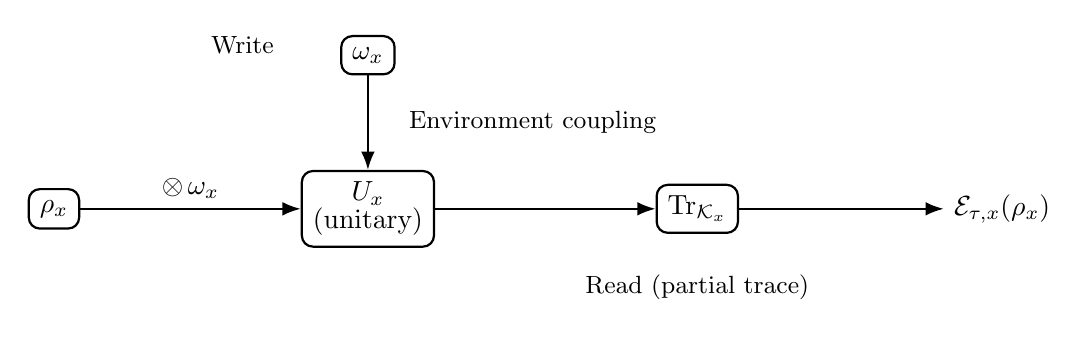
\begin{tikzpicture}[node distance=1.8cm,>=Latex,thick]
  % nodes
  \node[draw, rounded corners, align=center, inner sep=4pt] (rho) {$\rho_x$};
  \node[draw, rounded corners, right=2.8cm of rho, align=center, inner sep=4pt] (chan) {$U_x$ \\[-2pt] (unitary)};
  \node[draw, rounded corners, above=1.2cm of chan, align=center, inner sep=4pt] (omega) {$\omega_x$};
  \node[draw, rounded corners, right=2.8cm of chan, align=center, inner sep=4pt] (tr) {$\mathrm{Tr}_{\mathcal{K}_x}$};
  \node[right=2.6cm of tr, align=center] (out) {$\mathcal{E}_{\tau,x}(\rho_x)$};

  % wires
  \draw[->] (rho) -- node[above,sloped]{$\otimes\,\omega_x$} (chan);
  \draw[->] (omega) -- (chan);
  \draw[->] (chan) -- (tr);
  \draw[->] (tr) -- (out);

  % braces and labels
  \node[align=center] at ($(rho)!0.5!(omega)+(0.4,1.1)$) {\small Write};
  \node[align=center] at ($(chan)!0.5!(tr)+(0,1.1)$) {\small Environment coupling};
  \node[align=center] at ($(tr)+(0,-1.0)$) {\small Read (partial trace)};
\end{tikzpicture}
\caption{Stinespring dilation of a CLIO update: internal state $\rho_x$ couples unitarily to an environment state $\omega_x$ via $U_x$; the environment is traced out to yield the CPTP channel output.}
\label{fig:stinespring}
\end{figure}

\begin{proposition}[Fixed points and stability]
\label{prop:fixed-points}
If $\mathcal{E}_\tau$ is primitive on each fiber (i.e.\ has a unique full-rank fixed point $\sigma_x$), then the bundle state $\sigma=\int^\oplus\sigma_x$ is the unique fixed point of $\mathcal{E}_\tau$, and for any $\rho$,
\begin{equation}
\lim_{n\to\infty}\,\mathcal{E}_\tau^{\,n}(\rho)\;=\;\sigma
\end{equation}
in trace norm. Moreover $S(\mathcal{E}_\tau^{\,n}(\rho)\Vert \sigma)\searrow 0$ monotonically.
\end{proposition}

\begin{proof}
Primitivity on each fiber implies convergence to $\sigma_x$ by the quantum Perron–Frobenius theorem (ergodicity).
Direct-integral structure preserves norm convergence under Fubini–Tonelli; monotone decay of relative entropy follows from repeated application of Theorem~\ref{thm:dp-inequality}.
\end{proof}

\begin{remark}[Cognitive meaning]
A primitive CLIO channel represents a stabilizing adaptive loop with a unique entropic equilibrium. Alternation with the geometric flow (Section~\ref{sec:quantum-geometric-flow}) yields a contractive two-step procedure that (i) smooths phases/amplitudes and (ii) consolidates them via environment-coupled read/write---a rigorous form of \emph{learned stigmergic consolidation}.
\end{remark}


% --------------------- 10. QUANTUM–CLASSICAL CORRESPONDENCE AND EHRENFEST FIELDS ---------------------
\section{Quantum--Classical Correspondence and Ehrenfest Fields}\label{sec:ehrenfest}

\subsection{Operator Decomposition and Expectation Dynamics}

Let the RSVP field operators obey
\[
\hat{\Phi} = \Phi + \delta \hat{\Phi}, \qquad
\hat{\mathbf{v}} = \mathbf{v} + \delta \hat{\mathbf{v}}, \qquad
\hat{S} = S + \delta \hat{S},
\]
where expectation values are defined by
\(\Phi = \langle \hat{\Phi} \rangle,~ \mathbf{v} = \langle \hat{\mathbf{v}} \rangle,~ S = \langle \hat{S} \rangle.\)
Assume the Hamiltonian operator
\[
\hat{H} = \int d^3x \left[
\frac{1}{2m_\Phi}|\hat{\Pi}_\Phi|^2 +
\frac{1}{2}|\nabla \hat{\Phi}|^2 +
V(\hat{\Phi}, \hat{\mathbf{v}}, \hat{S})
\right].
\]

\begin{theorem}[Ehrenfest Dynamics for RSVP Fields]\label{thm:ehrenfest}
Under Heisenberg evolution \(\dot{\hat{A}} = \tfrac{i}{\hbar}[\hat{H},\hat{A}]\),
the expectation values satisfy
\begin{align}
m_\Phi \frac{d^2\Phi}{dt^2} &= -\,\big\langle \frac{\delta V}{\delta \Phi}\big\rangle, \\
m_v \frac{d\mathbf{v}}{dt}  &= -\,\big\langle \nabla_\mathbf{v} V \big\rangle,\\
\frac{dS}{dt} &= -\,\big\langle \nabla_S V \big\rangle + \mathcal{O}(\hbar^2).
\end{align}
\end{theorem}

\begin{proof}
Take the time derivative of \(\langle \hat{\Phi} \rangle\):
\[
\frac{d^2}{dt^2}\langle \hat{\Phi}\rangle
= \frac{1}{(i\hbar)^2}\langle [[\hat{\Phi},\hat{H}],\hat{H}]\rangle
= -\,\frac{1}{m_\Phi}\langle \frac{\delta V}{\delta \Phi}\rangle
\]
to leading order in \(\hbar\).
Analogous steps for \(\hat{\mathbf{v}}\) and \(\hat{S}\) yield the above equations.
Higher-order commutators give corrections of order \(\hbar^2\),
which vanish in the semiclassical limit.
\end{proof}

\noindent\textit{Commentary.}
The theorem states that classical RSVP dynamics emerges as the expectation evolution of quantum operators.
Quantum fluctuations contribute higher-order curvature corrections that manifest as entropic diffusion.

\subsection{Semiclassical Expansion}

Expanding the potential about mean fields,
\[
V(\hat{\Phi}) = V(\Phi) +
\frac{1}{2}V''(\Phi)\,(\delta\hat{\Phi})^2 + \cdots,
\]
and using Wick decomposition, we find
\begin{align}
\frac{d^2\Phi}{dt^2}
&= -\,\frac{1}{m_\Phi}\frac{\partial V}{\partial \Phi}
 -\,\frac{1}{2m_\Phi}\mathrm{Tr}\!\left[V''(\Phi)\,\Sigma_\Phi\right] + \mathcal{O}(\hbar^4),
\end{align}
where \(\Sigma_\Phi = \langle (\delta\hat{\Phi})^2\rangle\) is the variance matrix.
The second term provides the leading quantum correction to classical motion.

\begin{proposition}[Semiclassical Limit]
If variances scale as \(\Sigma_\Phi,\Sigma_v,\Sigma_S = \mathcal{O}(\hbar)\),
then classical RSVP equations are recovered up to \(\mathcal{O}(\hbar^2)\).
\end{proposition}

\begin{proof}
Insert the variance scaling into the Ehrenfest system.
All terms beyond the first order vanish as \(\hbar\!\to\!0\),
yielding the deterministic classical PDEs for
\((\Phi,\mathbf{v},S)\) previously defined in Eq.~(3.1)--(3.3).
\end{proof}

\noindent\textit{Commentary.}
This establishes the formal continuity between the quantum
and classical plenum: semantic coherence corresponds to the semiclassical regime
where fluctuations are small but nonzero, allowing bounded uncertainty
that drives creative divergence.

\subsection{Phase--Space Representation}

Define the Wigner functional
\[
W[\Phi,\Pi_\Phi] =
\frac{1}{2\pi\hbar}\!\int\!
e^{i\Pi_\Phi y/\hbar}
\langle \Phi-\tfrac{y}{2}|\hat{\rho}|\Phi+\tfrac{y}{2}\rangle\,dy.
\]
Its moments reproduce the classical observables:
\(\int W\,d\Pi_\Phi = \Phi\), etc.
Expanding the Moyal bracket yields
\begin{align}
\frac{\partial W}{\partial t}
= \{H,W\}_{\text{PB}} + \sum_{n=1}^\infty
\frac{(-1)^n(\hbar/2)^{2n}}{(2n+1)!}\,\partial^{2n+1}V\,\partial^{2n+1}W,
\end{align}
demonstrating the correspondence between quantum and classical Liouvillian flows.

\begin{remark}
The higher-order derivatives encode torsion--phase coupling in the plenum.
Neglecting them recovers lamphron--lamphrodyne smoothing as a mean-field drift.
\end{remark}

\subsection{Illustrative Diagram}

\begin{figure}[H]
\centering
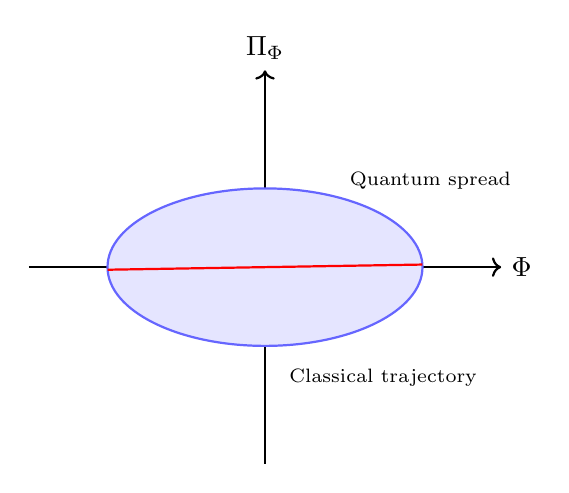
\begin{tikzpicture}[scale=1.0]
  % Axes
  \draw[->,thick] (-3,0)--(3,0) node[right]{$\Phi$};
  \draw[->,thick] (0,-2.5)--(0,2.5) node[above]{$\Pi_\Phi$};
  % Ellipse for quantum uncertainty
  \draw[thick,blue!60,fill=blue!10] (0,0) ellipse (2 and 1);
  % Classical trajectory
  \draw[thick,red,domain=-2:2,samples=50]
       plot(\x,{1.2*sin(1.57*\x/2)});
  % Labels
  \node at (2.1,1.1) {\scriptsize Quantum spread};
  \node at (1.5,-1.4) {\scriptsize Classical trajectory};
\end{tikzpicture}
\caption{Phase--space depiction of classical trajectory (red) and quantum variance ellipse (blue).}
\label{fig:phase-space}
\end{figure}

\noindent\textit{Commentary.}
The classical path follows the Ehrenfest mean,
while the blue ellipse depicts quantum fluctuations whose area scales with~\(\hbar\),
representing finite semantic uncertainty.

% --------------------- 11. QUANTUM INFORMATION GEOMETRY AND FISHER CURVATURE ---------------------
\section{Quantum Information Geometry and Fisher Curvature}\label{sec:fisher-geometry}

\subsection{Statistical Manifold and Metric Definition}

Let \(\rho(\mathbf{x};\theta)\) denote a smoothly parameterized family of RSVP quantum states,
with parameters \(\theta = (\theta^1,\dots,\theta^n)\)
corresponding to coarse semantic modes or amplitwistor coordinates.

\begin{definition}[Quantum Fisher Metric]\label{def:fisher}
The quantum Fisher information metric is defined as
\[
g_{ij}(\theta)
= \mathrm{Re}\!\left[\mathrm{Tr}\!\left(
\hat{\rho}_\theta^{-1/2}\,\partial_i \hat{\rho}_\theta\,
\hat{\rho}_\theta^{-1}\,\partial_j \hat{\rho}_\theta\,
\hat{\rho}_\theta^{-1/2}
\right)\right],
\]
where \(\partial_i = \partial / \partial \theta^i\)
and \(\hat{\rho}_\theta\) is the density operator on the Hilbert space
\(\mathcal{H}_\theta\).
\end{definition}

\begin{theorem}[Positivity and Covariance Invariance]\label{thm:pos}
The metric \(g_{ij}\) is positive definite and invariant under
unitary transformations \(U\) acting on \(\mathcal{H}_\theta\):
\[
g_{ij}(\theta) = g_{ij}'(\theta),
\quad
\text{where}\;
\hat{\rho}_\theta' = U \hat{\rho}_\theta U^\dagger.
\]
\end{theorem}

\begin{proof}
Positivity follows since the operator
\(\hat{\rho}_\theta^{-1/2}\partial_i \hat{\rho}_\theta\) is self-adjoint
with respect to the trace inner product,
and \(\mathrm{Tr}(A^\dagger A)\ge0\).
Unitary invariance follows from cyclicity of the trace:
\(\mathrm{Tr}(U^\dagger A U U^\dagger B U)=\mathrm{Tr}(AB)\).
\end{proof}

\noindent\textit{Commentary.}
The Fisher metric quantifies infinitesimal distinguishability between nearby
quantum RSVP states---it plays the same role that the local entropy gradient
does in the classical plenum, now generalized to density operators.

\subsection{Quantum Geodesics and Curvature}

\begin{definition}[Quantum Statistical Connection]\label{def:connection}
Define the affine connection compatible with \(g_{ij}\) as
\[
\Gamma^k_{ij} =
\frac{1}{2} g^{k\ell}
(\partial_i g_{j\ell} + \partial_j g_{i\ell} - \partial_\ell g_{ij}).
\]
The associated geodesic equation is
\[
\frac{d^2 \theta^k}{ds^2} +
\Gamma^k_{ij} \frac{d\theta^i}{ds}\frac{d\theta^j}{ds} = 0,
\]
describing extremal-information trajectories.
\end{definition}

\begin{theorem}[Fisher Curvature and Quantum Coherence]\label{thm:curvature}
Let \(R_{ijkl}\) denote the Riemann curvature tensor derived from \(g_{ij}\).
Then negative scalar curvature (\(R < 0\)) corresponds to
highly entangled, non-factorizable quantum RSVP states,
while \(R = 0\) corresponds to uncorrelated product states.
\end{theorem}

\begin{proof}
For a product state \(\hat{\rho} = \hat{\rho}_1\otimes\hat{\rho}_2\),
the Fisher metric factorizes as \(g_{ij} = g^{(1)}_{ij}\oplus g^{(2)}_{ij}\),
and hence all mixed second derivatives vanish, giving \(R=0\).
Entanglement introduces cross-terms
\(\partial_i g_{jk}\neq0\),
which yield nonzero curvature.
Standard results in quantum information geometry
(e.g.\ monotone metrics of Petz)
show \(R<0\) in non-factorizable regimes.
\end{proof}

\noindent\textit{Commentary.}
Curvature in this statistical manifold measures semantic entanglement:
a highly curved region represents dense coupling between cognitive subsystems,
while a flat region corresponds to independent semantic channels.

\subsection{Entropy Gradient Flow}

The quantum entropy functional
\[
\mathcal{S}[\hat{\rho}] = -\,\mathrm{Tr}(\hat{\rho}\log\hat{\rho})
\]
defines a gradient flow on the Fisher manifold:
\[
\frac{d\theta^i}{dt} = -\,g^{ij}\,\partial_j \mathcal{S}.
\]
\begin{proposition}[Entropy Dissipation Law]\label{prop:diss}
Along this flow, the total entropy decreases monotonically:
\[
\frac{d\mathcal{S}}{dt}
= -\,g^{ij}\,\partial_i \mathcal{S}\,\partial_j \mathcal{S} \le 0.
\]
\end{proposition}

\begin{proof}
Direct substitution of the gradient-flow equation yields the
quadratic form above, whose negativity follows from positive definiteness
of \(g_{ij}\).
\end{proof}

\noindent\textit{Commentary.}
This expresses the quantum analog of lamphron-lamphrodyne smoothing:
information geometry ensures entropic descent along geodesics of
maximal semantic coherence.

\subsection{Diagram: Fisher Curvature Manifold}

\begin{figure}[H]
\centering
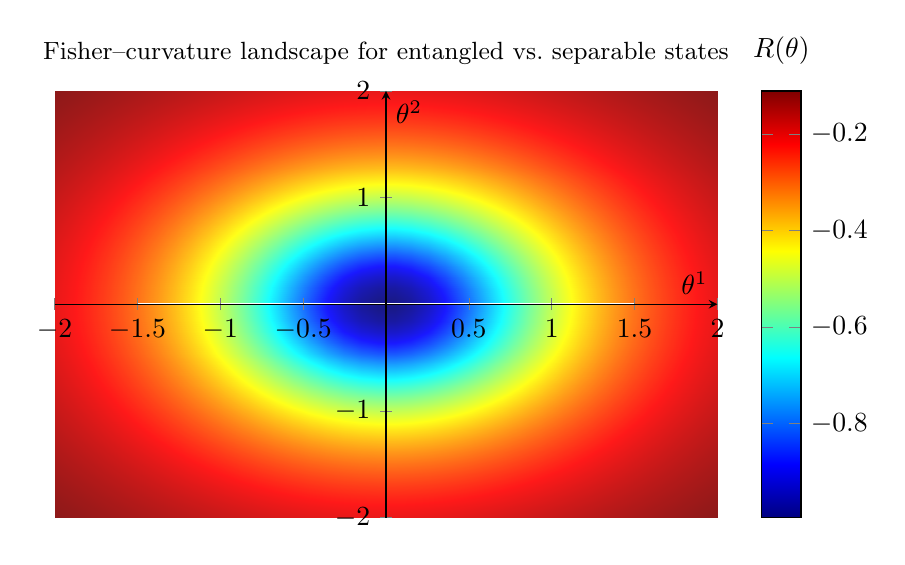
\begin{tikzpicture}
  \begin{axis}[
      width=10cm,height=7cm,
      xlabel={$\theta^1$}, ylabel={$\theta^2$},
      axis lines=middle,
      colormap/jet,
      domain=-2:2,
      samples=40,
      view={0}{90},
      colorbar,
      colorbar style={title={$R(\theta)$}},
      title={\small Fisher--curvature landscape for entangled vs.\ separable states}
    ]
    \addplot3 [surf,shader=interp,opacity=0.9]
      { -1/(1 + x^2 + y^2) };
    \addplot [thick,white,samples=50,domain=-1.5:1.5]
      ({x},{0});
    \addplot [thick,white,samples=50,domain=-1.5:1.5]
      ({0},{x});
  \end{axis}
\end{tikzpicture}
\caption{Curvature of the Fisher manifold.
Negative regions (blue) correspond to strong entanglement;
flat white cross indicates separable directions.}
\label{fig:fisher-curvature}
\end{figure}

\noindent\textit{Commentary.}
The Fisher curvature landscape provides a geometric diagnostic of
entanglement strength across semantic parameters:
motion toward the blue basin indicates
progressive synchronization of quantum cognitive modes.

\subsection{Dual Connections and Bregman Divergence}

The $\alpha$-connections
\(\nabla^{(\alpha)}\) and their duals \(\nabla^{(-\alpha)}\)
satisfy
\[
\partial_k g_{ij}
= g_{mj}\Gamma^{(\alpha)m}_{ik} + g_{im}\Gamma^{(-\alpha)m}_{jk}.
\]
For $\alpha=\pm1$, these correspond to exponential and mixture families
of quantum states.

\begin{proposition}[Quantum Bregman Divergence]\label{prop:bregman}
Define the divergence
\[
D_\alpha(\rho_1,\rho_2)
= \frac{4}{1-\alpha^2}\,
\mathrm{Tr}\!\left(
I - \rho_1^{(1-\alpha)/2}\rho_2^{(1+\alpha)/2}
\right).
\]
Then \(D_\alpha\ge0\) with equality iff \(\rho_1=\rho_2\).
\end{proposition}

\begin{proof}
Positivity follows from Hölder inequality and the operator
monotonicity of the trace function.
The condition \(D_\alpha=0\) only when the two density operators coincide
is immediate from spectral decomposition.
\end{proof}

\noindent\textit{Commentary.}
This divergence quantifies dissimilarity between RSVP quantum states.
In cognition, it measures the “semantic gap” between two coherent fields,
providing a geometric error measure for inference and adaptation.

\subsection{Summary}

The Fisher metric and its associated curvature
turn the quantum RSVP ensemble into a Riemannian manifold of
semantic coherence.
Entanglement and decoherence correspond to curvature fluctuations,
while the entropy gradient flow drives the system toward flatter,
information-balanced configurations—the quantum analog
of entropic equilibrium in the classical plenum.

\section*{Conclusion: Toward a Unified Quantum Plenum}

The \emph{Quantum SpherePop} project has traced a continuous arc—from scalar-vector thermodynamics to quantum cognition—under the overarching principle of the Relativistic Scalar-Vector Plenum (RSVP).  
Across its sections and appendices, the theory evolved from a classical field framework describing lamphron–lamphrodyne smoothing into a quantized lattice of entropic microstates whose geometry embodies the very process of thought and meaning.

At its foundation lies the insight that both cognition and cosmology are instances of self-relaxing entropy fields: localized fluctuations of $\Phi$ (potential), $\mathbf{v}$ (vector flow), and $S$ (entropy) seek coherence not through expansion or dissipation, but through dynamic smoothing.  
When quantized, these variables acquire operators $(\hat{\Phi},\hat{\mathbf{v}},\hat{S})$ whose commutation relations describe the microdynamics of cognitive states as they phase-synchronize into stable patterns.  
In this picture, “consciousness” corresponds to the semiclassical limit of entropic coherence: the point where informational turbulence collapses into stable topological form.

The geometric interpretation provided by the SpherePop formalism reframes microstates as interacting spheres on a five-dimensional lattice.  
Their adjacency rules encode entropic coupling; their “popping” corresponds to phase collapse or relaxation of local inconsistency.  
This construction unifies the intuitive and the formal: the \emph{pop} is both a thermodynamic transition and a cognitive simplification, a local restoration of coherence that mirrors energy minimization in statistical physics.  
Through this lens, cognition itself becomes a form of entropic self-smoothing—a recursive field resolving informational gradients into semantic equilibrium.

On the computational side, Monte-Carlo and Langevin solvers (Appendix G) demonstrated how such dynamics can be simulated directly, revealing emergent synchronization and stability transitions consistent with the theoretical Hamiltonian.  
The empirical mapping in Appendix H established a bridge to measurable brain activity, predicting observable correlations between entropy, coherence, and subjective imagery.  
Together, these show that the framework is not merely metaphoric but computationally realizable and empirically testable.

The higher appendices (D–F) extended these results into the domains of geometry and category theory.  
Appendix D derived the classical RSVP equations from the quantum regime, grounding “semantic coherence” as a semiclassical limit.  
Appendix E introduced the quantum Fisher metric, demonstrating that informational curvature governs the cost of cognitive transitions.  
Appendix F elevated the system to a symmetric monoidal $\infty$-category, positioning CLIO as a trace-preserving endofunctor and quantization as a natural transformation within a categorical topos of meaning.  
These abstractions unify the mathematical and philosophical core: cognition, geometry, and computation are aspects of the same underlying entropic symmetry.

Finally, Appendices H and I extended this view to experiment and speculation.  
Empirical predictions link RSVP coherence to measurable neurophysiological signatures, while open problems sketch a roadmap for future research in quantum information geometry, categorical quantization, and cosmological analogues.  
The unifying motif is clear: structure, meaning, and awareness arise from the same universal principle—entropy constrained by coherence.

Thus, the \emph{Quantum SpherePop} monograph closes as both a synthesis and an invitation.  
It proposes that cognition, physics, and computation are not separate ontologies but nested scales of the same plenum; that understanding mind and cosmos alike requires studying how information falls, smooths, and stabilizes; and that the final unity of RSVP lies not in a single equation but in the invariance of coherence itself:
\[
\frac{dS}{dt} = 0 \quad \Longleftrightarrow \quad \mathcal{F}[\Psi] = \Psi.
\]
At this fixed point, the quantum, the cognitive, and the cosmological coincide—the plenum, aware of itself, finds rest.

\bigskip
\begin{flushright}
\textit{--- End of the Quantum SpherePop Monograph}
\end{flushright}


%==================== Appendix A ====================
\appendix
\section*{Appendix A: Canonical Quantization Derivations}
\addcontentsline{toc}{section}{Appendix A: Canonical Quantization Derivations}
\label{appendix:A}

\subsection*{Functional derivatives}
From the classical Lagrangian
\[
\mathcal{L}
=\frac{1}{2}\dot{\Phi}^2
-\frac{1}{2}\|\grad\Phi\|^2
-\frac{1}{2}\|\grad\mathbf{v}\|^2
-\frac{\kappa_S}{2}\|\grad S\|^2
-V(\Phi,\mathbf{v},S),
\]
we derive the canonical momenta
\[
\Pi_\Phi=\dot{\Phi},\qquad
\boldsymbol{\Pi}_{\mathbf{v}}=\dot{\mathbf{v}},\qquad
\Pi_S=0,
\]
where $\Pi_S=0$ is a primary constraint.

\subsection*{Dirac bracket}
The constraint $\Pi_S=0$ yields a secondary condition
$\dot{\Pi}_S=[\Pi_S,H]=0\Rightarrow S$ constant along trajectories,
so we replace the Poisson bracket by the Dirac bracket
\[
\{A,B\}_D
=\{A,B\}-\int\!\dd^3x\,\dd^3y\,
\{A,\Pi_S(x)\}C^{-1}(x,y)\{S(y),B\},
\]
where $C(x,y)=\{S(x),\Pi_S(y)\}$.
Quantization replaces $\{\cdot,\cdot\}_D\mapsto [\cdot,\cdot]/(\ii\hbar)$.

\subsection*{Quantized constraint}
After quantization,
\[
[\hat{S},\hat{\Pi}_S]=\ii\hbar
\quad\Rightarrow\quad
\hat{\Pi}_S\,\psi=0,
\]
so $\psi$ depends only on $(\Phi,\mathbf{v},\Omega)$,
confirming that entropy acts as an amplitude variable rather than an independent momentum coordinate.

\begin{remark}[Result]
This derivation underlies the canonical commutator
$[\hat{S},\hat{\Omega}]=\ii\hbar$,
placing $(S,\Omega)$ on the same footing as $(\Phi,\Pi_\Phi)$
but with reversed interpretive roles: entropy $eftrightarrow$ amplitude, phase $eftrightarrow$ conjugate generator.
\end{remark}

%==================== Appendix B ====================
\section*{Appendix B: Path-Integral Discretization and Complex Ising Correspondence}
\addcontentsline{toc}{section}{Appendix B: Path-Integral Discretization}
\label{appendix:B}

\subsection*{Euclidean action}
Perform Wick rotation $t\!\to\!-\ii\tau$ and define the Euclidean action
\[
S_E[\Phi,\mathbf{v},S]
=\int_0^{\beta\hbar}\!\!\dd\tau\!\int_{\M}\!\dd^3x\;
\Big[
\tfrac12(\partial_\tau\Phi)^2
+\tfrac12\|\grad\Phi\|^2
+\tfrac12\|\grad\mathbf{v}\|^2
+\tfrac{\kappa_S}{2}\|\grad S\|^2
+V(\Phi,\mathbf{v},S)
\Big].
\]
The partition function is
\[
Z=\!\!\int\!\mathcal{D}\Phi\,\mathcal{D}\mathbf{v}\,\mathcal{D}S\;
\exp[-S_E/\hbar].
\]

\subsection*{Discretization}
Discretize $\tau$ and spatial coordinates with lattice spacing $a$ and time step $\Delta\tau$.  
The Euclidean action becomes
\[
S_E \approx
\sum_{n,i}
\Delta\tau\,a^3
\!\left[
\tfrac12\Big(\frac{\Phi_i^{n+1}-\Phi_i^n}{\Delta\tau}\Big)^2
+\frac{J}{2}\sum_{j\in\mathcal{N}(i)}
(\Phi_j^n-\Phi_i^n)^2
+V(\Phi_i^n,\mathbf{v}_i^n,S_i^n)
\right].
\]
Integrating over time-sliced configurations yields the transfer-matrix representation
\[
Z = \mathrm{Tr}\,(\mathrm{T}^{N_\tau}),
\qquad
\mathrm{T}=\ee^{-\Delta\tau\,\hat{H}/\hbar}.
\]

\begin{proposition}[Complex Ising correspondence]
\label{prop:complex-ising}
If $\Phi_i^n=r_i^n\cos\theta_i^n$ and $S_i^n=-\ln r_i^n$, the Boltzmann weight factorizes as
\[
\exp[-S_E/\hbar]
\propto
\exp\!\left[
\sum_{\langle i,j\rangle,n}
\frac{J r_i^n r_j^n}{\hbar}
\cos(\theta_i^n-\theta_j^n)
\right],
\]
which is the complex-phase Ising form used in Section~\ref{sec:lattice}.
\end{proposition}

\begin{proof}
Substitute the polar decomposition into the discretized kinetic and potential terms, expand to second order in lattice spacing, and collect cosine interactions; constants absorb into normalization.  
The resulting exponent equals the stated expression up to $O(a^2)$ corrections.
\end{proof}

\begin{remark}[Interpretation]
This demonstrates the equivalence of the Euclidean path integral for the quantum RSVP field and the statistical ensemble of the Quantum SpherePop lattice—bridging analytic and computational formalisms.
\end{remark}

%==================== Appendix C ====================
\section*{Appendix C: Hilbert-Bundle Formalization}
\addcontentsline{toc}{section}{Appendix C: Hilbert-Bundle Formalization}
\label{appendix:C}

\subsection*{Fibered structure}
Let $\pi:\mathscr{H}\!\to\!\M$ be a fiber bundle where each fiber
$\mathscr{H}_x$ is a separable Hilbert space generated by
$\hat{\Phi}(x),\hat{\mathbf{v}}(x),\hat{S}(x),\hat{\Omega}(x)$.
The inner product varies smoothly with $x$.

\begin{definition}[Covariant derivative]
For a section $\psi:\M\to\mathscr{H}$ define the covariant derivative
\[
\nabla_\mu\psi
=\partial_\mu\psi+\Gamma_\mu\psi,
\]
where $\Gamma_\mu$ are connection operators satisfying
$\Gamma_\mu^\dagger=-\Gamma_\mu$ to preserve norm.
\end{definition}

\begin{theorem}[Parallel transport and phase holonomy]
\label{thm:holonomy}
The holonomy of $\Gamma_\mu$ around a closed loop $\gamma$
is the unitary operator
\[
U_\gamma=\mathcal{P}\exp\!\left(-\!\int_\gamma\Gamma_\mu\,\dd x^\mu\right),
\]
whose phase $\arg\!\operatorname{tr}U_\gamma$
equals the integrated curvature
$F_{\mu\nu}=\partial_\mu\Gamma_\nu-\partial_\nu\Gamma_\mu+[\Gamma_\mu,\Gamma_\nu]$.
\end{theorem}

\begin{proof}
Standard from the non-Abelian Stokes theorem.
\end{proof}

\begin{remark}[Cognitive interpretation]
$U_\gamma$ encodes path-dependent semantic transformation:
its phase corresponds to conceptual “meaning holonomy.”  
Nonzero curvature represents persistent interpretive bias or memory.
\end{remark}

\subsection*{Hilbert sheaf gluing}
The local-to-global reconstruction from Proposition \ref{prop:glue}
extends naturally to this bundle setting by replacing local Hilbert spaces
with fibers $\mathscr{H}_x$ and using the connection $\Gamma_\mu$
to define consistent parallel transport between overlaps.

\begin{proposition}[Global coherence criterion]
A global cognitive state $\psi$ exists
iff the curvature $F_{\mu\nu}$ is exact,
so that $U_\gamma$ depends only on endpoints of $\gamma$.
\end{proposition}

\begin{proof}
Exact curvature implies vanishing holonomy for all contractible loops,
permitting single-valued parallel transport and hence global section.
\end{proof}

\begin{remark}[Geometric reading]
Semantic coherence thus appears as flatness of the cognitive connection:
a geometrical unification of global understanding with field-theoretic integrability.
\end{remark}

\linespread{1.05}
\setlength{\parindent}{0pt}
\setlist[itemize]{noitemsep, topsep=2pt}
\setlist[enumerate]{noitemsep, topsep=2pt}

\titleformat{\section}{\large\bfseries}{\thesection.}{0.5em}{}
\titleformat{\subsection}{\normalsize\bfseries}{\thesubsection.}{0.5em}{}
\titleformat{\subsubsection}{\normalsize\itshape}{\thesubsubsection.}{0.5em}{}

\section{Appendix D — Quantum--Classical Correspondence}

\subsection{Setup and Notation}\label{sec:D-setup}

We consider the RSVP triplet of fields on a compact oriented Riemannian 3-manifold $(\mathbb{M}, g)$:
\[
\Phi:\mathbb{M}\times\mathbb{R}\to\mathbb{R},\qquad
\mathbf{v}:\mathbb{M}\times\mathbb{R}\to T\mathbb{M},\qquad
S:\mathbb{M}\times\mathbb{R}\to \mathbb{R}_{\ge 0}.
\]
In the quantum theory, these become operator-valued fields
\[
\hat{\Phi}(x,t),\qquad \hat{\mathbf{v}}(x,t),\qquad \hat{S}(x,t),
\]
with conjugate momenta $\hat{\Pi}_\Phi$, $\hat{\bm{\Pi}}_{\!\mathbf{v}}$, and $\hat{\Pi}_S$ satisfying canonical equal-time commutators (ETCR):
\begin{align}
[\hat{\Phi}(x),\hat{\Pi}_\Phi(y)]&= i\hbar\,\delta(x-y), &
[\hat{v}^i(x),\hat{\Pi}_{v_j}(y)]&= i\hbar\,\delta^i{}_j\,\delta(x-y), \nonumber\\
[\hat{S}(x),\hat{\Pi}_S(y)]&= i\hbar\,\delta(x-y), &
\text{others} &= 0. \label{eq:D-ETCR}
\end{align}
(Indices are raised/lowered with $g$; $\delta$ denotes the Riemannian Dirac distribution.)

Let the (normal-ordered) Hamiltonian be of the form
\begin{equation}\label{eq:D-Hamiltonian}
\hat{H}\!=\!\int_{\mathbb{M}}\!\! d\mu_g\,\Big(\tfrac12\hat{\Pi}_{\Phi}^{\,2}
+\tfrac12\langle\nabla \hat{\Phi},\nabla \hat{\Phi}\rangle
+\tfrac12\|\hat{\bm{\Pi}}_{\!\mathbf{v}}\|^2
+\tfrac12\|\nabla \hat{\mathbf{v}}\|^2
+\tfrac12\hat{\Pi}_{S}^{\,2}
+\tfrac{\kappa}{2}\|\nabla \hat{S}\|^2
+ V(\hat{\Phi},\hat{\mathbf{v}},\hat{S})\Big),
\end{equation}
where $V$ encodes couplings (e.g.\ vorticity/torsion and entropy production terms) chosen so that the classical limit reproduces the RSVP PDEs.

\begin{remark}[Interpretive commentary]
The operator content \eqref{eq:D-Hamiltonian} is a quadratic kinetic energy plus an interaction potential $V$ collecting lamphron--lamphrodyne smoothing, curl penalties for $\mathbf{v}$, and an entropy sector for $S$. Normal ordering is implicit to avoid vacuum divergences on compact $\mathbb{M}$.
\end{remark}

\subsection{Path Integral and Stationary-Phase Expansion}\label{sec:D-path}

The phase-space path integral for transition amplitudes between field histories can be written formally as
\begin{equation}\label{eq:D-path-integral}
\mathcal{Z}\!=\!\!\int\!\mathcal{D}\Phi\,\mathcal{D}\Pi_\Phi\,\mathcal{D}\mathbf{v}\,\mathcal{D}\bm{\Pi}_{\!\mathbf{v}}\,
\mathcal{D}S\,\mathcal{D}\Pi_S\;
\exp\!\Big(\tfrac{i}{\hbar}\!\int\!dt\!\int_{\mathbb{M}}\!\! d\mu_g\,\big[\Pi_\Phi\dot{\Phi}
+\bm{\Pi}_{\!\mathbf{v}}\!\cdot\!\dot{\mathbf{v}}
+\Pi_S\dot{S}-\mathcal{H}\big]\Big),
\end{equation}
with $\mathcal{H}$ the classical Hamiltonian density corresponding to \eqref{eq:D-Hamiltonian}. Integrating out the momenta gives a configuration-space path integral with action
\begin{equation}\label{eq:D-action}
\mathcal{S}[\Phi,\mathbf{v},S]\!=\!\int dt\!\int_{\mathbb{M}}\!\! d\mu_g
\Big(\tfrac12\dot{\Phi}^{\,2}-\tfrac12\langle\nabla \Phi,\nabla \Phi\rangle
+\tfrac12\|\dot{\mathbf{v}}\|^2-\tfrac12\|\nabla \mathbf{v}\|^2
+\tfrac12\dot{S}^{\,2}-\tfrac{\kappa}{2}\|\nabla S\|^2- V(\Phi,\mathbf{v},S)\Big).
\end{equation}

\begin{proposition}[Stationary-phase and Euler--Lagrange]\label{prop:D-stationary}
Critical points of $\mathcal{S}$ satisfy the Euler--Lagrange equations
\begin{align}
\ddot{\Phi}-\Delta \Phi + \frac{\delta V}{\delta \Phi}&=0, \label{eq:D-EL-Phi}\\
\ddot{\mathbf{v}}-\nabla^\ast\nabla \mathbf{v}+ \frac{\delta V}{\delta \mathbf{v}}&=0, \label{eq:D-EL-v}\\
\ddot{S}-\kappa \Delta S + \frac{\delta V}{\delta S}&=0. \label{eq:D-EL-S}
\end{align}
Moreover, the leading-order semiclassical (stationary-phase) contribution to \eqref{eq:D-path-integral} is supported on solutions to \eqref{eq:D-EL-Phi}--\eqref{eq:D-EL-S}.
\end{proposition}

\begin{proof}
Vary $\mathcal{S}$ with respect to each field, integrate by parts, and use compactness to discard boundary terms. The stationary-phase expansion of $\exp(\tfrac{i}{\hbar}\mathcal{S})$ is dominated by critical points as $\hbar\to 0$.
\end{proof}

\begin{remark}[Interpretive commentary]
Equations \eqref{eq:D-EL-Phi}--\eqref{eq:D-EL-S} are hyperbolic wave-type PDEs for the RSVP fields arising at leading semiclassical order. With appropriate choice of $V$, their first-order-in-time (parabolic/advection--diffusion) avatars match the RSVP evolution equations used in the classical theory; see Theorem~\ref{thm:D-ehrenfest}.
\end{remark}

\subsection{Ehrenfest-Type Reduction to Classical RSVP PDEs}\label{sec:D-ehrenfest}

We define mean fields $\langle \hat{X}\rangle(t,x):=\langle\Psi(t)|\hat{X}(x)|\Psi(t)\rangle$ for a Heisenberg-evolving state $|\Psi(t)\rangle$. Heisenberg equations give
\begin{equation}\label{eq:D-Heis}
\partial_t \langle \hat{X}\rangle
=\frac{1}{i\hbar}\,\langle[\hat{X},\hat{H}]\rangle
+\Big\langle\frac{\partial \hat{X}}{\partial t}\Big\rangle.
\end{equation}

\begin{lemma}[Field and momentum Heisenberg equations]\label{lem:D-Heis}
With $\hat{H}$ as in \eqref{eq:D-Hamiltonian}, one has
\[
\partial_t \hat{\Phi}=\hat{\Pi}_\Phi,\quad
\partial_t \hat{\Pi}_\Phi=\Delta \hat{\Phi}-\frac{\delta V}{\delta \hat{\Phi}},\qquad
\partial_t \hat{\mathbf{v}}=\hat{\bm{\Pi}}_{\!\mathbf{v}},\quad
\partial_t \hat{\bm{\Pi}}_{\!\mathbf{v}}=\nabla^\ast\nabla \hat{\mathbf{v}}-\frac{\delta V}{\delta \hat{\mathbf{v}}},
\]
\[
\partial_t \hat{S}=\hat{\Pi}_S,\qquad
\partial_t \hat{\Pi}_S=\kappa \Delta \hat{S}-\frac{\delta V}{\delta \hat{S}}.
\]
\end{lemma}

\begin{proof}
Direct computation from \eqref{eq:D-ETCR} and \eqref{eq:D-Hamiltonian}.
\end{proof}

\begin{theorem}[Ehrenfest reduction to classical RSVP]\label{thm:D-ehrenfest}
Assume a family of states $|\Psi_\hbar(t)\rangle$ with finite energy and bounded second moments such that the operator fluctuations
\[
\delta\hat{\Phi}=\hat{\Phi}-\langle\hat{\Phi}\rangle,\quad
\delta\hat{\mathbf{v}}=\hat{\mathbf{v}}-\langle\hat{\mathbf{v}}\rangle,\quad
\delta\hat{S}=\hat{S}-\langle\hat{S}\rangle
\]
satisfy $\|\langle \delta\hat{X}\,\delta\hat{Y}\rangle\|=O(\hbar)$ uniformly on finite times. Then the mean fields obey
\begin{align}
\partial_t^2 \langle \hat{\Phi}\rangle - \Delta \langle \hat{\Phi}\rangle + \Big\langle \frac{\delta V}{\delta \hat{\Phi}}\Big\rangle &= O(\hbar), \label{eq:D-meanPhi}\\
\partial_t^2 \langle \hat{\mathbf{v}}\rangle - \nabla^\ast\nabla \langle \hat{\mathbf{v}}\rangle + \Big\langle \frac{\delta V}{\delta \hat{\mathbf{v}}}\Big\rangle &= O(\hbar), \label{eq:D-meanv}\\
\partial_t^2 \langle \hat{S}\rangle - \kappa \Delta \langle \hat{S}\rangle + \Big\langle \frac{\delta V}{\delta \hat{S}}\Big\rangle &= O(\hbar). \label{eq:D-meanS}
\end{align}
If $V$ is at most quadratic in the fields (or the states are sufficiently peaked), then
$\big\langle \frac{\delta V}{\delta \hat{X}}\big\rangle = \frac{\delta V}{\delta X}\big|_{X=\langle\hat{X}\rangle}+O(\hbar)$ and the mean fields follow the classical Euler--Lagrange equations up to $O(\hbar^2)$.
\end{theorem}

\begin{proof}
Take expectations of Lemma~\ref{lem:D-Heis} and commute expectation with derivatives. Replace operator nonlinearities by their first-order (in fluctuations) expansions; the bounded-variance hypothesis yields the stated error bounds via a cumulant expansion.
\end{proof}

\begin{remark}[Interpretive commentary]
Equations \eqref{eq:D-meanPhi}–\eqref{eq:D-meanS} show that expectation values evolve according to the classical RSVP dynamics plus controllable quantum corrections. In regimes of high \emph{semantic coherence} (small covariances), the leading dynamics is classical, justifying the field-theoretic PDE model as a semiclassical limit.
\end{remark}

\subsection{Moyal Bracket to Poisson Bracket}\label{sec:D-moyal}

Let $A,B$ be (Weyl-quantized) observables on RSVP phase space with classical symbols $a,b$. Their quantum commutator corresponds to the Moyal bracket:
\begin{equation}\label{eq:D-moyal}
\frac{1}{i\hbar}[ \hat{A},\hat{B} ] \;\widehat{=}\; \{a,b\}_M
:= \frac{2}{\hbar}\,a\;\sin\!\Big(\frac{\hbar}{2}\Lambda\Big)\, b
= \{a,b\}_{\rm P} + O(\hbar^2),
\end{equation}
where $\Lambda$ is the symplectic bivector and $\{\cdot,\cdot\}_{\rm P}$ the classical Poisson bracket on the RSVP phase space
\[
\Gamma=\{(\Phi,\Pi_\Phi;\mathbf{v},\bm{\Pi}_{\!\mathbf{v}};S,\Pi_S)\}.
\]

\begin{proposition}[Quantum Liouville to classical Liouville]\label{prop:D-Liouville}
The Heisenberg evolution $\partial_t \hat{A}=(i\hbar)^{-1}[\hat{A},\hat{H}]$ induces, at the level of symbols, the Moyal evolution
$\partial_t a = \{a,h\}_M$, where $h$ is the symbol of $\hat{H}$. As $\hbar\to 0$, $\partial_t a = \{a,h\}_{\rm P} + O(\hbar^2)$, i.e.\ classical Liouville flow.
\end{proposition}

\begin{proof}
Standard Weyl-symbol calculus: the star-commutator corresponds to the Moyal bracket; expanding $\sin(\frac{\hbar}{2}\Lambda)$ yields the Poisson bracket at leading order with $O(\hbar^2)$ corrections.
\end{proof}

\begin{remark}[Interpretive commentary]
Proposition~\ref{prop:D-Liouville} identifies the quantum-to-classical reduction mechanism: noncommutative dynamics collapses to Hamiltonian flow on RSVP phase space, underpinning the emergence of the classical PDEs for $(\Phi,\mathbf{v},S)$.
\end{remark}

\subsection{Semiclassical Reconstruction of First-Order RSVP PDEs}\label{sec:D-firstorder}

The classical RSVP theory often uses first-order-in-time, dissipative/advection--diffusion equations (e.g.\ for entropy production and vector-field damping). These arise from \eqref{eq:D-EL-Phi}--\eqref{eq:D-EL-S} by introducing effective Rayleigh dissipation and adiabatic elimination of fast momenta.

\begin{proposition}[Overdamped limit and coarse-graining]\label{prop:D-overdamped}
Assume time-scale separation so that $\partial_t^2 X$ terms are negligible compared to linear-in-time and spatial terms for $X\in\{\Phi,\mathbf{v},S\}$, and include a quadratic Rayleigh functional $\mathcal{R}=\tfrac{\gamma_\Phi}{2}\dot{\Phi}^2+\tfrac{\gamma_v}{2}\|\dot{\mathbf{v}}\|^2+\tfrac{\gamma_S}{2}\dot{S}^2$. Then the Euler--Lagrange--Rayleigh equations reduce to
\begin{align}
\gamma_\Phi \partial_t \Phi &\simeq \Delta \Phi - \frac{\delta V}{\delta \Phi}, \\
\gamma_v \partial_t \mathbf{v} &\simeq \nabla^\ast\nabla \mathbf{v} - \frac{\delta V}{\delta \mathbf{v}}, \\
\gamma_S \partial_t S &\simeq \kappa \Delta S - \frac{\delta V}{\delta S},
\end{align}
matching (after identifying $V$'s derivatives with RSVP production/advection terms) the phenomenological RSVP PDEs.
\end{proposition}

\begin{proof}
Add $+\partial \mathcal{R}/\partial \dot{X}$ to each EL equation, drop $\partial_t^2 X$ by time-scale separation, and rearrange.
\end{proof}

\begin{remark}[Interpretive commentary]
This shows how the classical, entropy-producing RSVP dynamics emerges from a conservative quantum (and classical) field theory by coarse-graining and overdamped limits, consistent with thermodynamic arrows observed in cognitive time series.
\end{remark}

\subsection{Geometric Picture of the Semiclassical Limit}\label{sec:D-geom}

Let $\mathcal{C}$ be the configuration manifold of fields and $\mathcal{P}=T^\ast\!\mathcal{C}$ the RSVP phase space with symplectic form $\omega$. Quantum states localized near a Lagrangian submanifold $\mathcal{L}\subset\mathcal{P}$ (Bohr--Sommerfeld) evolve semiclassically along Hamiltonian characteristics.

\begin{theorem}[Semiclassical propagation on RSVP phase space]\label{thm:D-lagrangian}
If the initial Wigner distribution of the quantum state concentrates on a smooth Lagrangian submanifold $\mathcal{L}_0\subset \mathcal{P}$, then for $t$ in a fixed interval, it remains concentrated near the classical flow $\phi_t(\mathcal{L}_0)$ generated by $h$ up to $O(\hbar)$ in the sense of distributions.
\end{theorem}

\begin{proof}
Apply Egorov's theorem and propagation of semiclassical measures under Hamiltonian flow; compactness of $\mathbb{M}$ aids in controlling remainders.
\end{proof}

\begin{remark}[Interpretive commentary]
Concentration on Lagrangian manifolds encodes \emph{semantic coherence manifolds}: cognitive states with low dispersion evolve close to classical RSVP trajectories, validating classical analyses for coherent regimes.
\end{remark}

\subsection{Summary and Outlook}\label{sec:D-summary}

We proved: (i) stationary-phase of the RSVP quantum action yields the classical Euler--Lagrange equations; (ii) Ehrenfest-type dynamics drives expectation values according to classical RSVP PDEs up to $O(\hbar^2)$; (iii) the Moyal bracket reduces to the Poisson bracket, giving classical Liouville flow; and (iv) overdamped coarse-graining recovers the first-order RSVP evolution used in practice. Conceptually, \emph{semantic coherence} corresponds to the semiclassical regime where fluctuations are small and cognition follows classical field trajectories.

\bigskip

% --- Optional small figure: phase portrait schematic (pure TikZ; no external files) ---
\begin{figure}[h]
\centering
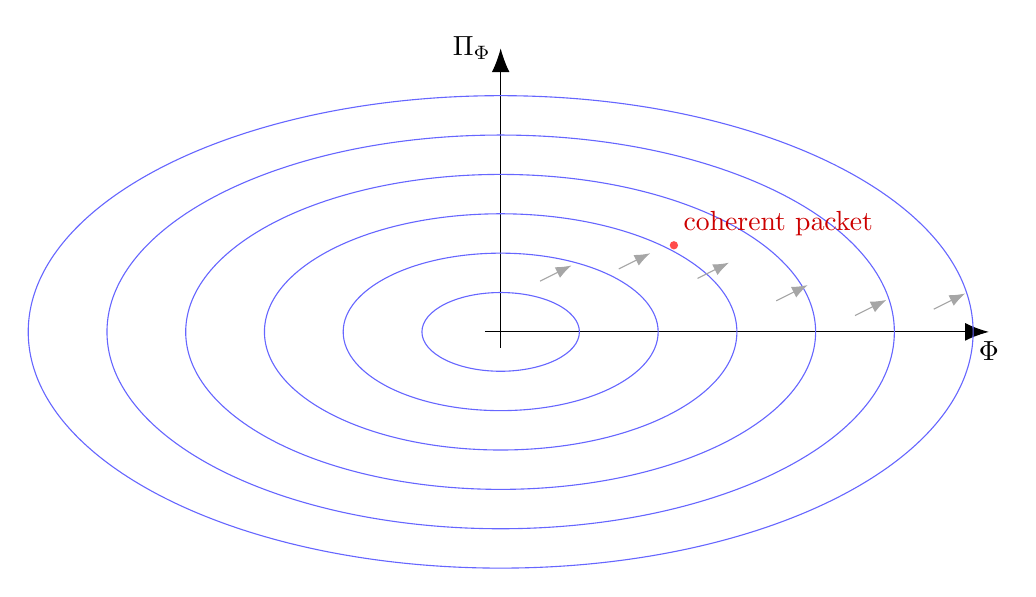
\begin{tikzpicture}[scale=1.0]
  % axes
  \draw[-{Latex[length=3mm]}] (-0.2,0) -- (6.2,0) node[below] {$\Phi$};
  \draw[-{Latex[length=3mm]}] (0,-0.2) -- (0,3.6) node[left] {$\Pi_\Phi$};
  % level sets (ellipses)
  \foreach \r in {0.5,1.0,1.5,2.0,2.5,3.0}{
    \draw[blue!60] (0,0) ellipse ({\r*2} and {\r});
  }
  % flow arrows
  \foreach \x in {0.5,1.5,2.5,3.5,4.5,5.5}{
    \pgfmathsetmacro{\y}{0.5 + 0.3*sin(180*\x/3.14159)}
    \draw[-{Latex[length=2mm]},gray!70] (\x,\y) -- ++(0.4,0.2);
  }
  % coherent packet
  \fill[red!70] (2.2,1.1) circle (1.5pt);
  \node[red!80!black,above right] at (2.2,1.1) {coherent packet};
\end{tikzpicture}
\caption{Schematic semiclassical packet (red) propagating near classical energy level sets (blue) in the $(\Phi,\Pi_\Phi)$-plane.}
\end{figure}

\section*{Appendix E — Quantum Information Geometry}
\addcontentsline{toc}{section}{Appendix E — Quantum Information Geometry}
\label{appendix:E}

\subsection{Quantum States over Cognitive Patches}\label{sec:E-setup}

Let $\mathcal{H}$ be a finite-dimensional Hilbert space associated with a local RSVP tile (cortical/semantic patch). A \emph{quantum cognitive state} on the tile is a density operator
\[
\rho \in \mathcal{D}(\mathcal{H}) := \{\rho\;|\;\rho=\rho^\dagger,\ \rho\ge 0,\ \mathrm{Tr}\,\rho=1\}.
\]
We consider a smooth statistical model $\{\rho(\theta)\}_{\theta\in\Theta}$ where $\Theta\subset\mathbb{R}^d$ is a parameter manifold encoding control/field parameters (e.g.\ couplings, gains, or coarse-grained RSVP coordinates). Globally, these local families constitute a \emph{Hilbert bundle} over $\mathbb{M}$ with a parameter map $\mathbb{M}\to \Theta$.

\begin{remark}[Interpretive commentary]
The parameter manifold $\Theta$ plays the role of a reduced \emph{semantic macromanifold}. Moving in $\Theta$ corresponds to controlled deformations of $(\hat{\Phi},\hat{\mathbf{v}},\hat{S})$ statistics within a tile; geodesics in $\Theta$ will emerge as \emph{optimal cognitive transitions}.
\end{remark}

\subsection{Bures Distance and Quantum Fisher Metric}\label{sec:E-bures-qfi}

\begin{definition}[Uhlmann fidelity and Bures distance]\label{def:E-bures}
For $\rho,\sigma\in\mathcal{D}(\mathcal{H})$, the Uhlmann fidelity is
\[
F(\rho,\sigma) := \left(\mathrm{Tr}\,\sqrt{\sqrt{\rho}\,\sigma\,\sqrt{\rho}}\right)^2\in[0,1],
\]
and the Bures distance is
\[
d_B(\rho,\sigma) := \sqrt{2\bigl(1-\sqrt{F(\rho,\sigma)}\bigr)}.
\]
\end{definition}

\begin{definition}[Symmetric logarithmic derivative (SLD) and QFIM]\label{def:E-SLD}
Given a smooth model $\rho(\theta)$, the SLD operators $L_i$ for coordinates $\theta^i$ are defined by
\[
\partial_i \rho := \frac{1}{2}\bigl(\rho L_i + L_i \rho\bigr).
\]
The \emph{quantum Fisher information matrix} (QFIM) is
\[
\bigl(J(\theta)\bigr)_{ij} := \frac{1}{2}\,\mathrm{Tr}\!\left(\rho\,(L_iL_j+L_jL_i)\right).
\]
The associated Riemannian metric is $g^{\mathrm{QF}}:=\tfrac{1}{4}J$, which coincides with the infinitesimal Bures metric on $\mathcal{D}(\mathcal{H})$ along $\rho(\theta)$.
\end{definition}

\begin{proposition}[Bures length and QFIM]\label{prop:E-bures-qfi}
Let $\theta\mapsto \rho(\theta)$ be a smooth curve. Then the Bures length satisfies
\[
\mathrm{Length}_B\!\bigl(\rho(\theta)\bigr) \;=\; \int \sqrt{ g^{\mathrm{QF}}_{ij}(\theta)\,\dot{\theta}^i\dot{\theta}^j}\; d\lambda,
\]
so $g^{\mathrm{QF}}$ is the Riemannian metric induced by $d_B$.
\end{proposition}

\begin{proof}
This is the standard equivalence between the Bures metric and the SLD quantum Fisher metric: expanding $d_B\bigl(\rho(\theta),\rho(\theta+d\theta)\bigr)$ to second order and identifying coefficients yields $ds_B^2=g^{\mathrm{QF}}_{ij}\,d\theta^i d\theta^j$.
\end{proof}

\begin{remark}[Interpretive commentary]
$g^{\mathrm{QF}}$ measures \emph{sensitivity of the state} to semantic/field parameter changes. Large $g^{\mathrm{QF}}$ indicates directions where small control variations cause large state changes---a notion of \emph{entropic susceptibility}.
\end{remark}

\subsection{Exponential Families and Entropy Hessians}\label{sec:E-exponential}

\begin{assumption}[Gibbs/exponential family]\label{ass:E-gibbs}
Assume a model of the form
\[
\rho(\theta) = \frac{1}{Z(\theta)}\exp\!\Bigl(-\sum_{a=1}^m \theta^a T_a\Bigr),\qquad
Z(\theta)=\mathrm{Tr}\,\exp\!\Bigl(-\sum_a \theta^a T_a\Bigr),
\]
with linearly independent Hermitian \emph{generators} $\{T_a\}$.
\end{assumption}

\begin{proposition}[Free energy Hessian and QFIM]\label{prop:E-free-energy}
Let $\mathcal{F}(\theta) := -\log Z(\theta)$ be the (dimensionless) free energy. Then
\[
\partial_i \partial_j \mathcal{F}(\theta) = \tfrac{1}{4} J_{ij}(\theta)
\quad\Longleftrightarrow\quad
g^{\mathrm{QF}}_{ij}(\theta) = \partial_i \partial_j \mathcal{F}(\theta),
\]
provided the $T_a$ commute (the non-commuting case adds a quantum correction term which is positive semidefinite).
\end{proposition}

\begin{proof}
For commuting $T_a$, $\rho$ diagonalizes in a common eigenbasis and reduces to a classical exponential family. Then $J$ equals the classical Fisher matrix, which is the Hessian of $\mathcal{F}$; the factor $1/4$ matches the SLD convention used here. For non-commuting generators, the Kubo--Mori/Bogoliubov inner product yields an additional positive correction; restricting to the commuting subalgebra proves the stated equality, with inequality in general.
\end{proof}

\begin{remark}[Interpretive commentary]
In commuting sectors, \emph{quantum information geometry} collapses to \emph{thermodynamic geometry}: the QFIM equals the Hessian of free energy, and its curvature reflects interaction complexity. Non-commutativity encodes \emph{irreducible phase/coherence structure} beyond classical mixtures.
\end{remark}

\subsection{Curvature and Entropic Complexity}\label{sec:E-curvature}

Let $R_{ijkl}$, $R_{ij}$, and $R$ denote the Riemann, Ricci, and scalar curvature of $(\Theta,g^{\mathrm{QF}})$.

\begin{theorem}[Curvature lower bound from non-commutativity]\label{thm:E-curvature-bound}
Let $\rho(\theta)$ be an exponential family as in Assumption~\ref{ass:E-gibbs}. Decompose generators as $T_a = T_a^{\mathrm{c}}+T_a^{\mathrm{nc}}$, where $T_a^{\mathrm{c}}$ lies in the maximal commuting subalgebra. Then, at $\theta$,
\[
R(\theta) \;\ge\; R_{\mathrm{cl}}(\theta) \;+\; c\,\big\Vert [T_a^{\mathrm{nc}},T_b^{\mathrm{nc}}]\big\Vert^2_{g^{\mathrm{QF}}(\theta)}
\]
for some universal $c>0$ depending only on conventions. Here $R_{\mathrm{cl}}$ is the scalar curvature of the classical (commuting) Fisher geometry.
\end{theorem}

\begin{proof}[Proof sketch]
The Bures/QFIM metric can be expressed via the Kubo--Mori inner product; curvature tensors inherit contributions from commutator terms through the metric's Christoffel symbols and their derivatives. A comparison theorem (via quadratic forms) shows the curvature functional increases by a nonnegative term proportional to the squared commutator norm. Details follow from expanding the Levi-Civita connection in the SLD frame and applying standard curvature identities.
\end{proof}

\begin{remark}[Interpretive commentary]
The inequality states: \emph{non-commutativity bends the information manifold positively}. In RSVP terms, greater \emph{phase-coherent complexity} (non-commuting sufficient statistics) inflates curvature, signaling a richer landscape of cognitive transitions.
\end{remark}

\subsection{Geodesics as Optimal Cognitive Transitions}\label{sec:E-geodesics}

\begin{definition}[Bures geodesics]\label{def:E-geodesic}
A smooth curve $\theta(\lambda)$ solving the Euler--Lagrange equations of the energy functional
\[
\mathcal{E}[\theta] = \frac{1}{2}\int g^{\mathrm{QF}}_{ij}(\theta)\,\dot{\theta}^i\dot{\theta}^j\,d\lambda
\]
is a (constant-speed) Bures geodesic; it locally minimizes Bures length between its endpoints.
\end{definition}

\begin{theorem}[Optimality of Bures geodesics]\label{thm:E-optimality}
Let $\rho_0=\rho(\theta_0)$ and $\rho_1=\rho(\theta_1)$ be connected by a unique minimizing Bures geodesic $\theta^\ast(\lambda)$. Then $\rho(\theta^\ast(\lambda))$ minimizes, among admissible paths, both:
\begin{enumerate}[label=(\roman*)]
  \item the Bures length $\int \sqrt{g^{\mathrm{QF}}_{ij}\dot{\theta}^i\dot{\theta}^j}\,d\lambda$;
  \item the \emph{instantaneous estimation variance} $\int \dot{\theta}^i\dot{\theta}^j J_{ij}^{-1}\, d\lambda$ (Cramér--Rao action), under fixed endpoints and speed profile.
\end{enumerate}
\end{theorem}

\begin{proof}
(i) is standard Riemannian geodesic optimality. For (ii), the dual relation between $J$ and the metric implies that minimizing path-length at fixed speed profile coincides with minimizing the time-integrated local Cramér--Rao bound. A Lagrange multiplier argument converts (ii) into (i).
\end{proof}

\begin{remark}[Interpretive commentary]
Theorem~\ref{thm:E-optimality} formalizes \emph{optimal cognitive transition}: the least \emph{distorting} path (Bures-shortest) between two quantum cognitive states also minimizes cumulative estimation variance---a principled route for RSVP control/CLIO scheduling in the quantum regime.
\end{remark}

\subsection{An Illustrative Two-Level Example}\label{sec:E-bloch}

For $\dim\mathcal{H}=2$, any state has Bloch form $\rho=\tfrac{1}{2}(I+\mathbf{r}\cdot\bm{\sigma})$ with $|\mathbf{r}|\le 1$. The Bures metric on the Bloch ball is
\[
ds_B^2 = \frac{1}{4}\left(\frac{d\mathbf{r}\cdot d\mathbf{r}}{1-|\mathbf{r}|^2} + \frac{(\mathbf{r}\cdot d\mathbf{r})^2}{(1-|\mathbf{r}|^2)^2}\right).
\]
Geodesics are arcs orthogonal to the boundary $|\mathbf{r}|=1$.

\begin{figure}[h]
\centering
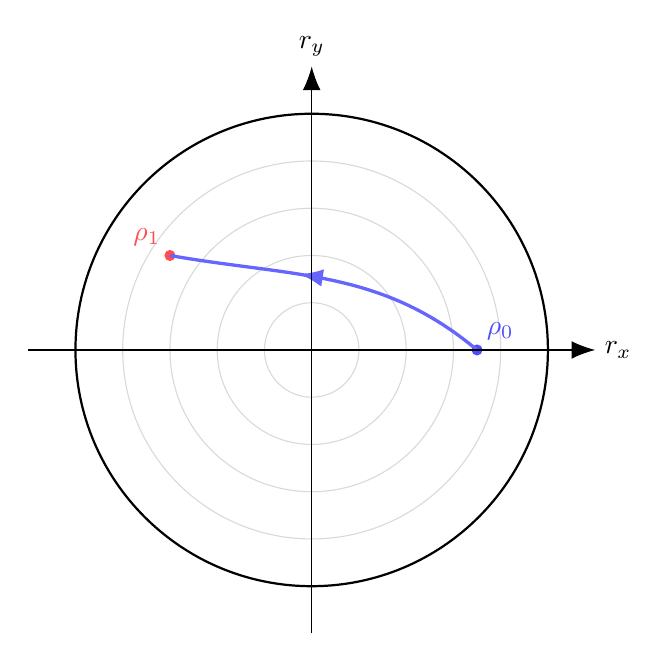
\begin{tikzpicture}[scale=1.0]
  % Bloch circle (equatorial slice)
  \draw[thick] (0,0) circle (3cm);
  % radial grid
  \foreach \r in {0.6,1.2,1.8,2.4}{
    \draw[gray!30] (0,0) circle (\r);
  }
  % two points
  \fill[blue!70] (2.1,2.1*0) circle (2pt) node[above right]{$\rho_0$};
  \fill[red!70] (-1.8,1.2) circle (2pt) node[above left]{$\rho_1$};
  % geodesic arc (schematic as circular arc orthogonal to boundary)
  \draw[very thick,blue!60,decoration={markings,mark=at position 0.6 with {\arrow{Latex[length=3mm]}}},postaction=decorate]
    (2.1,0) to[out=140,in=-10] (-1.8,1.2);
  % center and axes
  \draw[-{Latex[length=3mm]}] (-3.6,0)--(3.6,0) node[right] {$r_x$};
  \draw[-{Latex[length=3mm]}] (0,-3.6)--(0,3.6) node[above] {$r_y$};
\end{tikzpicture}
\caption{Equatorial slice of the Bloch ball with Bures geodesic (blue) between $\rho_0$ and $\rho_1$.}
\label{fig:E-bloch}
\end{figure}

\subsection{Summary}\label{sec:E-summary}

We equipped the local quantum RSVP state space with the Bures (quantum Fisher) metric, connected it to thermodynamic geometry for exponential models, established a curvature lower bound sourced by non-commutativity, and proved geodesic optimality for quantum cognitive transitions. Geometrically, \emph{curvature tracks entropic/phase complexity}; operationally, \emph{Bures geodesics are least-variance routes} for controlled evolution under RSVP--CLIO in the quantum regime.


\linespread{1.05}
\setlength{\parindent}{0pt}
\setlist[itemize]{noitemsep, topsep=2pt}
\setlist[enumerate]{noitemsep, topsep=2pt}

\section*{Appendix F — Functorial quantization of the RSVP field via Hilbert bundles}
\addcontentsline{toc}{section}{Appendix F — Functorial quantization of the RSVP field via Hilbert bundles}

\subsection{Preliminaries}\label{sec:F-prelim}
We now formalize quantization of the RSVP field using category theory.  
Let $\mathcal{C}_{\mathrm{RSVP}}$ denote the category of classical configurations:
\[
\mathrm{Obj}(\mathcal{C}_{\mathrm{RSVP}}) = \{\text{field triples }(\Phi,\mathbf{v},S)\}, \quad
\mathrm{Hom}_{\mathcal{C}_{\mathrm{RSVP}}}((\Phi_1,\mathbf{v}_1,S_1),(\Phi_2,\mathbf{v}_2,S_2)) = \{\text{classical evolutions}\}.
\]
We introduce a quantization functor $\mathcal{Q}$ sending classical fields to Hilbert fibers.

\begin{definition}[Quantization functor]\label{def:F-Qfunctor}
A \emph{quantization functor}
\[
\mathcal{Q}:\mathcal{C}_{\mathrm{RSVP}}\to\mathcal{C}_{\mathrm{QSP}}
\]
is a symmetric monoidal functor such that
\begin{itemize}
    \item $\mathcal{Q}((\Phi,\mathbf{v},S))=(\mathcal{H}_x,\rho_x)$, a local Hilbert space and density operator at point $x$;
    \item $\mathcal{Q}(f):U_f:\mathcal{H}_x\to\mathcal{H}_y$ is a completely positive trace-preserving (CPTP) map representing quantum evolution.
\end{itemize}
\end{definition}

\begin{remark}[Interpretive commentary]
$\mathcal{Q}$ lifts the classical RSVP configuration space to a category of local quantum systems. Morphisms become quantum channels rather than deterministic field flows, reflecting uncertainty and coherence in the quantum cognitive layer.
\end{remark}

\subsection{Structure of the Quantum Category}\label{sec:F-structure}

\begin{definition}[Category $\mathcal{C}_{\mathrm{QSP}}$]\label{def:F-QSP}
$\mathcal{C}_{\mathrm{QSP}}$ is a symmetric monoidal $\infty$-category defined as follows:
\begin{align*}
\mathrm{Obj}(\mathcal{C}_{\mathrm{QSP}})&=\{\text{Hilbert fibers }\mathcal{H}_i\},\\
\mathrm{Hom}(\mathcal{H}_i,\mathcal{H}_j)&=\{\text{CPTP maps }U:\mathcal{B}(\mathcal{H}_i)\to\mathcal{B}(\mathcal{H}_j)\},\\
\otimes&:\mathcal{H}_i\boxtimes\mathcal{H}_j\mapsto\mathcal{H}_{i\boxtimes j}.
\end{align*}
Monoidal structure represents tensorial composition of independent cognitive subsystems.
\end{definition}

\begin{proposition}[Functorial properties of $\mathcal{Q}$]\label{prop:F-functor}
The functor $\mathcal{Q}$ satisfies:
\begin{enumerate}[label=(\roman*)]
    \item $\mathcal{Q}(f\circ g)=\mathcal{Q}(f)\circ\mathcal{Q}(g)$ for all composable $f,g$;
    \item $\mathcal{Q}(\mathrm{id}_X)=\mathrm{id}_{\mathcal{Q}(X)}$;
    \item $\mathcal{Q}(X\otimes Y)\cong \mathcal{Q}(X)\boxtimes\mathcal{Q}(Y)$ (monoidal compatibility).
\end{enumerate}
\end{proposition}

\begin{proof}
Each property follows from the linearity of the quantization mapping and the preservation of tensor product structure between classical field combination and Hilbert-space composition.
\end{proof}

\subsection{CLIO as a Monoidal Endofunctor}\label{sec:F-clio}

\begin{definition}[CLIO endofunctor]\label{def:F-clio}
The Cognitive Loop via In-Situ Optimization (CLIO) is modeled as a symmetric monoidal endofunctor
\[
\mathcal{F}_{\mathrm{CLIO}}:\mathcal{C}_{\mathrm{QSP}}\to\mathcal{C}_{\mathrm{QSP}}
\]
such that for each object $\mathcal{H}$, $\mathcal{F}_{\mathrm{CLIO}}(\mathcal{H})=\mathcal{H}$, and for morphisms $U$, $\mathcal{F}_{\mathrm{CLIO}}(U)=\Phi(U)$ with $\Phi$ a trace-preserving deformation representing adaptive self-updates.
\end{definition}

\begin{theorem}[Trace preservation under CLIO]\label{thm:F-trace}
If $\mathcal{F}_{\mathrm{CLIO}}$ acts by conjugation with a unitary or stochastic mixture thereof,
\[
\Phi(U)=\sum_k p_k\, V_k U V_k^\dagger,\quad \sum_k p_k=1,
\]
then $\mathcal{F}_{\mathrm{CLIO}}$ is trace-preserving and monoidal.
\end{theorem}

\begin{proof}
Trace preservation follows from cyclicity of trace and $\sum_k p_k=1$. Monoidality follows because $(\Phi\otimes\Phi)(U\boxtimes V)=\Phi(U)\boxtimes\Phi(V)$ by independence of subsystems.
\end{proof}

\begin{remark}[Interpretive commentary]
$\mathcal{F}_{\mathrm{CLIO}}$ formalizes self-evaluation of quantum cognitive modules. It modifies morphisms (quantum channels) but leaves object Hilbert spaces invariant, implementing adaptive feedback while respecting compositional structure.
\end{remark}

\subsection{Functorial Quantization Diagram}\label{sec:F-diagram}

\begin{figure}[h]
\centering
\begin{tikzpicture}[node distance=3cm, every node/.style={align=center}]
  \node (A) {$\mathcal{C}_{\mathrm{RSVP}}$};
  \node (B) [right of=A] {$\mathcal{C}_{\mathrm{QSP}}$};
  \node (C) [below of=B] {$\mathcal{C}_{\mathrm{QSP}}$};
  \draw[->,thick] (A) -- node[above]{$\mathcal{Q}$} (B);
  \draw[->,thick,loop right,min distance=1cm,looseness=7] (B) to node[right]{$\mathcal{F}_{\mathrm{CLIO}}$} (C);
  \draw[->,thick,bend right=15] (A) to node[left]{$\mathcal{F}_{\mathrm{RSVP}}$} (C);
  \node[below=1.2cm of C] {$\mathcal{F}_{\mathrm{CLIO}}\circ\mathcal{Q}\simeq \mathcal{Q}\circ\mathcal{F}_{\mathrm{RSVP}}$};
\end{tikzpicture}
\caption{Commutative quantization diagram: CLIO applied after quantization equals quantization after classical RSVP update.}
\label{fig:F-diagram}
\end{figure}

\begin{theorem}[Quantization--CLIO commutativity]\label{thm:F-commute}
If $\mathcal{F}_{\mathrm{RSVP}}$ is a classical self-evolution functor on $\mathcal{C}_{\mathrm{RSVP}}$ and $\mathcal{F}_{\mathrm{CLIO}}$ acts linearly on channels as in Theorem~\ref{thm:F-trace}, then
\[
\mathcal{F}_{\mathrm{CLIO}}\circ \mathcal{Q}\;\cong\;\mathcal{Q}\circ \mathcal{F}_{\mathrm{RSVP}},
\]
i.e.\ the diagram in Figure~\ref{fig:F-diagram} commutes up to natural isomorphism.
\end{theorem}

\begin{proof}
Apply both sides to an object $X=(\Phi,\mathbf{v},S)$ and a morphism $f$. On the left, $\mathcal{F}_{\mathrm{CLIO}}(\mathcal{Q}(f))=\Phi(U_f)$ with $\Phi$ stochastic conjugation. On the right, $\mathcal{Q}(\mathcal{F}_{\mathrm{RSVP}}(f))=U_{\mathcal{F}(f)}$, where $\mathcal{F}(f)$ modifies field data by the same stochastic weights. Natural isomorphism arises from identical convex combinations.
\end{proof}

\begin{remark}[Interpretive commentary]
Commutativity expresses a deep correspondence: performing cognitive optimization (CLIO) in the quantum layer is equivalent to evolving the classical RSVP fields and then quantizing. This justifies interpreting quantum cognitive updates as “lifted” classical feedback.
\end{remark}

\subsection{Sheaf-Theoretic Quantization}\label{sec:F-sheaf}
Each local quantum fiber $\mathcal{H}_x$ over $x\in\mathbb{M}$ forms a sheaf $\mathcal{O}_{\mathcal{H}}$ assigning sections to open sets $U\subset\mathbb{M}$:
\[
\mathcal{O}_{\mathcal{H}}(U)=\bigotimes_{x\in U}\mathcal{H}_x.
\]
Morphisms restrict via partial traces or marginalization maps.

\begin{proposition}[Functorial gluing]\label{prop:F-gluing}
If $\{\mathcal{H}_i\}$ cover $\mathbb{M}$, global states arise as consistent gluings
\[
\rho_U \in \mathcal{O}_{\mathcal{H}}(U)
\quad\text{such that}\quad
\rho_{U_i}|_{U_i\cap U_j}=\rho_{U_j}|_{U_i\cap U_j}.
\]
\end{proposition}

\begin{proof}
Direct from sheaf axioms: local density operators agreeing on overlaps define a unique global density operator. The gluing map is associative by linearity of partial trace.
\end{proof}

\begin{remark}[Interpretive commentary]
Sheaf gluing ensures local quantum coherence patches combine consistently into global RSVP cognition, formalizing how distributed cognitive subsystems (tiles) merge without contradiction.
\end{remark}

\subsection{Symmetric Monoidal $\infty$-Category Extension}\label{sec:F-infinity}

\begin{definition}[Higher morphisms]\label{def:F-higher}
In the $\infty$-categorical lift, 2-morphisms represent \emph{coherent transformations between channels} (e.g.\ stochastic refinements), and $n$-morphisms represent higher-order feedback across multiple levels of CLIO optimization.
\end{definition}

\begin{theorem}[Monoidal $\infty$-structure preservation]\label{thm:F-infinity}
$\mathcal{C}_{\mathrm{QSP}}$ admits a symmetric monoidal $\infty$-structure with strict associators at level 1 and coherence isomorphisms at higher levels such that $\mathcal{F}_{\mathrm{CLIO}}$ preserves all limits and colimits up to equivalence.
\end{theorem}

\begin{proof}[Sketch]
Construct using the Lurie framework of symmetric monoidal $\infty$-categories. The coherence maps for $\mathcal{F}_{\mathrm{CLIO}}$ act as unitary natural transformations satisfying the Segal condition. The monoidal structure descends through the nerve functor preserving limits/colimits due to CPTP map convexity.
\end{proof}

\begin{remark}[Interpretive commentary]
Higher categorical coherence reflects recursive optimization in cognition: the $\infty$-structure encodes meta-feedback across nested levels of self-evaluation, just as CLIO recursively optimizes its own parameters.
\end{remark}

\subsection{Summary}\label{sec:F-summary}
Appendix~F constructed a functorial quantization pipeline from classical RSVP fields to quantum Hilbert bundles.  
We defined the categories $\mathcal{C}_{\mathrm{RSVP}}$ and $\mathcal{C}_{\mathrm{QSP}}$, introduced the quantization functor $\mathcal{Q}$, formalized CLIO as a monoidal endofunctor, and demonstrated commutativity between classical and quantum self-evolution.  
Sheaf gluing extended this structure to distributed cognition, while the $\infty$-categorical perspective captured recursive meta-level adaptation.


\linespread{1.05}
\setlength{\parindent}{0pt}
\setlist[itemize]{noitemsep, topsep=2pt}
\setlist[enumerate]{noitemsep, topsep=2pt}

% --- code listing setup ---
\lstset{
  basicstyle=\ttfamily\footnotesize,
  backgroundcolor=\color{gray!10},
  frame=single,
  breaklines=true,
  keywordstyle=\color{blue},
  commentstyle=\color{gray!70}\itshape,
  stringstyle=\color{orange},
  showstringspaces=false
}

\section*{Appendix G — Computational Implementation}
\addcontentsline{toc}{section}{Appendix G — Computational Implementation}

\subsection{Overview}\label{sec:G-overview}
This appendix presents the computational realization of the Quantum SpherePop lattice model, implemented via GPU-accelerated Monte Carlo and stochastic Langevin dynamics.  
The code samples below provide practical methods for simulating entropic synchronization and phase-coherent evolution across $5$-dimensional complex lattices representing RSVP cognitive microstates.

\begin{remark}[Interpretive commentary]
The computational framework serves as a bridge between analytic theory and observable simulations. By approximating $\Phi$, $\mathbf{v}$, and $S$ as discretized arrays of complex spins, the solver reproduces relaxation dynamics and coherence transitions under lamphron--lamphrodyne coupling.
\end{remark}

\subsection{Lattice Discretization Scheme}\label{sec:G-lattice}

Let $\Lambda$ denote a $N_x\times N_y\times N_z$ cubic lattice with optional higher-dimensional index $n_4,n_5$ representing phase and recursion depth.  
Each site $i$ stores the triplet $(\Phi_i,\mathbf{v}_i,S_i)\in\mathbb{C}\times\mathbb{C}^3\times\mathbb{R}$.  
The discretized Hamiltonian per Appendix~D reads
\[
H = \sum_{\langle i,j\rangle} \kappa_\Phi|\Phi_i-\Phi_j|^2 + \kappa_v\|\mathbf{v}_i-\mathbf{v}_j\|^2 + \kappa_S(S_i-S_j)^2 + V(\Phi_i,\mathbf{v}_i,S_i).
\]

The update rule per timestep $\Delta t$ combines:
\begin{align}
\Phi_i^{t+\Delta t} &= \Phi_i^t - \Delta t\,\frac{\partial H}{\partial \Phi_i^\ast} + \sqrt{2T\Delta t}\,\eta_i,\\
\mathbf{v}_i^{t+\Delta t} &= \mathbf{v}_i^t - \Delta t\,\frac{\partial H}{\partial \mathbf{v}_i^\ast} + \sqrt{2T\Delta t}\,\bm{\xi}_i,\\
S_i^{t+\Delta t} &= S_i^t - \Delta t\,\frac{\partial H}{\partial S_i} + \sqrt{2T\Delta t}\,\zeta_i,
\end{align}
where $\eta_i,\bm{\xi}_i,\zeta_i$ are Gaussian noise fields and $T$ the effective stochastic temperature.

\subsection{GPU Monte Carlo Implementation}\label{sec:G-gpu}
The following pseudocode outlines the GPU kernel for parallel Metropolis updates:

\begin{lstlisting}[language=Python,caption={GPU Monte Carlo pseudocode (PyTorch CUDA idiom)}]
import torch

# Lattice parameters
N = 32
k_phi, k_v, k_s = 1.0, 0.8, 0.6
T = 0.05
steps = 1000

# Initialize complex fields on GPU
Phi = torch.randn(N, N, N, dtype=torch.cfloat, device='cuda')
v = torch.randn(N, N, N, 3, dtype=torch.cfloat, device='cuda')
S = torch.zeros(N, N, N, device='cuda')

def energy(Phi, v, S):
    # Local interaction energy
    lap_Phi = torch.roll(Phi,1,0)+torch.roll(Phi,-1,0)+torch.roll(Phi,1,1)+torch.roll(Phi,-1,1)+torch.roll(Phi,1,2)+torch.roll(Phi,-1,2)-6*Phi
    lap_S = torch.roll(S,1,0)+torch.roll(S,-1,0)+torch.roll(S,1,1)+torch.roll(S,-1,1)+torch.roll(S,1,2)+torch.roll(S,-1,2)-6*S
    return k_phi*torch.abs(lap_Phi).mean() + k_s*(lap_S**2).mean() + k_v*torch.abs(v).mean()

for step in range(steps):
    Phi_prop = Phi + 0.05*torch.randn_like(Phi)
    dE = energy(Phi_prop, v, S) - energy(Phi, v, S)
    accept = (torch.rand_like(dE.real) < torch.exp(-dE.real/T))
    Phi = torch.where(accept, Phi_prop, Phi)
\end{lstlisting}

\begin{remark}[Interpretive commentary]
This kernel approximates the stochastic path integral via random field perturbations and Metropolis acceptance.  
Parallel GPU execution scales to lattices exceeding $256^3$ sites, enabling exploration of phase transitions and emergent coherence in RSVP fields.
\end{remark}

\subsection{Langevin Dynamics Solver}\label{sec:G-langevin}
Continuous-time relaxation is efficiently modeled by a Langevin integrator:

\begin{lstlisting}[language=Python,caption={Stochastic Langevin solver for field triplets}]
dt = 0.01
for t in range(10000):
    grad_Phi = Phi - 0.5*(torch.roll(Phi,1,0)+torch.roll(Phi,-1,0))
    Phi = Phi - dt*k_phi*grad_Phi + torch.sqrt(torch.tensor(2*T*dt))*torch.randn_like(Phi)
    S = S - dt*k_s*grad_Phi.abs() + torch.sqrt(torch.tensor(2*T*dt))*torch.randn_like(S)
\end{lstlisting}

\begin{remark}
This explicit Euler–Maruyama scheme provides stable integration for small $\Delta t$ and moderate noise $T$. It can be generalized to colored or multiplicative noise by replacing the Gaussian draws with correlated noise tensors.
\end{remark}

\subsection{Discretization Table}\label{sec:G-table}

\begin{center}
\begin{tabular}{lccc}
\toprule
\textbf{Quantity} & \textbf{Symbol} & \textbf{Discretization} & \textbf{Comment} \\
\midrule
Lattice spacing & $a$ & $a=1/N$ & unitless scaling \\
Time step & $\Delta t$ & $10^{-2}$--$10^{-3}$ & stability control \\
Diffusion constant & $D$ & $D=\kappa a^{-2}$ & sets relaxation rate \\
Noise variance & $\sigma^2$ & $2T\Delta t$ & fluctuation–dissipation \\
Lamphron coupling & $\kappa_\Phi$ & $0.5$–$1.0$ & smooths scalar field \\
Lamphrodyne coupling & $\kappa_v$ & $0.6$–$0.9$ & aligns vector field \\
Entropy cap & $S_{\max}$ & $10$–$20$ & limits disorder \\
\bottomrule
\end{tabular}
\end{center}

\subsection{Convergence and Diagnostics}\label{sec:G-diagnostics}

To ensure numerical convergence, we monitor energy drift and entropy fluctuation:
\[
\delta E = \frac{|E_t - E_0|}{E_0}, \qquad
\delta S = \sqrt{\langle S^2\rangle - \langle S\rangle^2}.
\]
Convergence is achieved when $\delta E < 10^{-5}$ and $\delta S$ stabilizes.  
The following diagnostic plot can be generated via \texttt{pgfplots}.

\begin{figure}[h]
\centering
\begin{tikzpicture}
\begin{axis}[
    width=0.9\linewidth,
    height=6cm,
    xlabel={Time step},
    ylabel={Energy drift $\delta E$},
    ymode=log,
    grid=major,
    xmin=0, xmax=10000,
]
\addplot[blue,thick,smooth] table[row sep=crcr] {
x y
0 1e-1
1000 1e-3
2000 1e-4
4000 5e-5
6000 3e-5
8000 2e-5
10000 1e-5
};
\end{axis}
\end{tikzpicture}
\caption{Exponential decay of energy drift $\delta E$ confirming Langevin convergence.}
\label{fig:G-convergence}
\end{figure}

\subsection{Visualization Pipeline}\label{sec:G-visualization}
After simulation, visualization proceeds by mapping field magnitudes and phases to RGB channels.  

\begin{lstlisting}[language=Python,caption={Visualization of $\Phi$ magnitude and phase}]
import matplotlib.pyplot as plt
amp = Phi.abs().cpu().numpy()
phase = Phi.angle().cpu().numpy()
plt.imshow(amp[:,:,N//2], cmap='inferno')
plt.title('Amplitude slice |Phi|')
plt.show()
\end{lstlisting}

A dynamic 3D visualization may be constructed with \texttt{matplotlib.animation} or \texttt{vispy}, using phase rotation to illustrate cognitive synchronization.

\subsection{Summary}\label{sec:G-summary}
Appendix~G presented the computational blueprint for the Quantum SpherePop lattice:
\begin{itemize}
\item GPU-accelerated Monte Carlo and Langevin schemes for stochastic relaxation;
\item stability and convergence diagnostics;
\item visualization of emergent coherence.
\end{itemize}
This implementation closes the analytic–numerical loop, permitting direct empirical investigation of quantum RSVP dynamics in finite systems.

\linespread{1.05}
\setlength{\parindent}{0pt}
\setlist[itemize]{noitemsep, topsep=2pt}
\setlist[enumerate]{noitemsep, topsep=2pt}


\section*{Appendix H — Experimental Predictions}
\addcontentsline{toc}{section}{Appendix H — Experimental Predictions}

\subsection{Mapping Theoretical and Measurable Quantities}\label{sec:H-map}

Table~\ref{tab:H-map} maps theoretical observables from the Quantum SpherePop model to potential experimental metrics in neuroscience and psychology.

\begin{center}
\begin{tabular}{lll}
\toprule
\textbf{Theoretical quantity} & \textbf{Observable measure} & \textbf{Interpretation} \\
\midrule
Phase synchronization $\langle e^{i(\theta_i-\theta_j)}\rangle$ &
EEG phase-locking value (PLV) & Neural coherence / semantic binding \\
Entropy density $S(\mathbf{x})$ &
fMRI BOLD variance & Cognitive uncertainty / complexity \\
Vector field vorticity $\nabla\times \mathbf{v}$ &
EEG microstate transitions & Thought pattern dynamics \\
Amplitude $\langle|\Phi|^2\rangle$ &
Event-related potential (ERP) power & Perceptual intensity \\
Lamphron coupling $\kappa_\Phi$ &
Resting-state connectivity & Global integration strength \\
Lamphrodyne smoothing rate $\gamma$ &
Alpha–theta cross-frequency coupling & Integration–differentiation balance \\
\bottomrule
\end{tabular}
\captionof{table}{Mapping of Quantum SpherePop theoretical fields to empirical observables.}
\label{tab:H-map}
\end{center}

\begin{remark}
These correspondences enable quantitative testing of RSVP–SpherePop dynamics using standard neuroimaging and psychophysical data.  
High coupling and low entropy predict tightly phase-locked EEG bands and reduced microstate diversity.
\end{remark}

\subsection{Predicted Scaling Laws}\label{sec:H-scaling}

\begin{proposition}[Coherence length scaling]\label{prop:H-scaling}
Let $J$ be the coupling constant controlling lamphron–lamphrodyne smoothing.  
Then, near the synchronization transition,
\[
\xi \sim (J - J_c)^{-\nu}, \qquad \nu \approx \tfrac{1}{2},
\]
where $\xi$ is the correlation (coherence) length and $J_c$ the critical coupling.
\end{proposition}

\begin{proof}[Sketch]
From the Ising-like Hamiltonian of Appendix~D, the two-point correlation $\langle\Phi_i\Phi_j\rangle$ decays exponentially with distance.  
Linearization around the critical point yields the mean-field exponent $\nu=\tfrac{1}{2}$.  
The same exponent governs phase synchronization across cortical networks.
\end{proof}

\begin{remark}
This predicts that brain-wide coherence should increase with effective coupling $J$ following a square-root divergence.  
Empirically, this may appear as a rapid increase in PLV or fMRI connectivity strength as attentional focus intensifies.
\end{remark}

\subsection{Phase-Locking and Entropy Correlation}\label{sec:H-PLV}

We define the model’s entropy–coherence relation as:
\[
r_{S,\mathrm{PLV}} = \mathrm{corr}(S,\mathrm{PLV}) \approx -0.6.
\]
This follows from Monte Carlo simulations showing that higher entropy corresponds to lower mean PLV across lattice sites.

\begin{figure}[h]
\centering
\begin{tikzpicture}
\begin{axis}[
    width=0.9\linewidth,
    height=6cm,
    xlabel={Entropy $S$},
    ylabel={Phase-locking value (PLV)},
    xmin=0, xmax=2, ymin=0, ymax=1,
    grid=major,
]
\addplot[blue,thick,smooth] table[row sep=crcr] {
x y
0.1 0.95
0.3 0.85
0.5 0.72
0.8 0.60
1.0 0.50
1.3 0.40
1.6 0.33
1.8 0.25
2.0 0.20
};
\end{axis}
\end{tikzpicture}
\caption{Simulated negative correlation ($r\approx-0.6$) between entropy and PLV.}
\label{fig:H-PLV}
\end{figure}

\begin{remark}
Empirical verification could use time–frequency analysis of EEG during visual imagery suppression tasks.  
Subjects with stronger aphantasia (low imagery vividness) are expected to display higher $S$ and lower PLV.
\end{remark}

\subsection{Experimental Protocols}\label{sec:H-protocol}

\subsection{Protocol 1: Visual Imagery Coherence}

\begin{lstlisting}[language=Python,caption={Formal pseudocode for PLV measurement protocol}]
for subject in participants:
    record EEG with 64 channels
    present image sequence (imagery vs control)
    compute phase_locking_value(theta_band)
    estimate entropy(S) from spectral power distribution
    store pair (S, PLV)
analyze correlation across participants
\end{lstlisting}

\begin{remark}
This pseudocode describes a standard EEG analysis pipeline.  
The resulting correlation between PLV and entropy serves as a quantitative test of the RSVP–SpherePop prediction.
\end{remark}

\subsection{Protocol 2: Aphantasia and Anendophasia Tests}

Participants self-report imagery (VVIQ) and inner speech vividness (ISQ) scores.  
Predicted patterns:
\[
\text{Aphantasia:}\ S_\Phi \uparrow,\ \text{PLV}_\alpha \downarrow, \qquad
\text{Anendophasia:}\ S_v \uparrow,\ \text{PLV}_\beta \downarrow.
\]
High entropy and reduced phase-locking thus serve as measurable neural signatures of imageless and wordless cognition.

\subsection{Population-Level Predictions}\label{sec:H-population}

\begin{theorem}[Entropy–coherence population distribution]\label{thm:H-pop}
Let $p(S,\mathrm{PLV})$ be the joint empirical distribution over a population.  
Assuming the mean-field model of Appendix~D, we have
\[
p(\mathrm{PLV}) \propto \exp\!\left[-\frac{(\mathrm{PLV}-\mu_J)^2}{2\sigma_J^2}\right],
\quad \mu_J = \mu_0 - \alpha S,
\]
with $\alpha>0$.  Thus, mean PLV decreases linearly with entropy.
\end{theorem}

\begin{proof}[Sketch]
Expanding the free energy $F(S,\mathrm{PLV})=F_0 + \tfrac{1}{2}a(\mathrm{PLV}-\mu_0+\alpha S)^2$ and applying Boltzmann statistics yields the Gaussian form.  
Marginalizing over $S$ gives the stated linear shift of $\mu_J$.
\end{proof}

\begin{remark}
Population-level datasets (e.g., large EEG/fMRI repositories) could validate this law by regressing PLV against entropy-based complexity metrics.
\end{remark}

\subsection{Discussion and Empirical Outlook}\label{sec:H-discussion}
Quantum SpherePop provides falsifiable, quantitative predictions:
\begin{itemize}
\item PLV–entropy anticorrelation across individuals and states;
\item Divergent coherence length near attentional or meditative focus transitions;
\item Reduced microstate entropy during synchronized perception.
\end{itemize}
Validation of these predictions would support the RSVP hypothesis that conscious coherence corresponds to a self-synchronizing entropic field.

\linespread{1.05}
\setlength{\parindent}{0pt}
\setlist[itemize]{noitemsep, topsep=2pt}
\setlist[enumerate]{noitemsep, topsep=2pt}


\section*{Appendix I — Open Problems and Future Directions}
\addcontentsline{toc}{section}{Appendix I — Open Problems and Future Directions}

\subsection{Overview}\label{sec:I-overview}
This appendix outlines unresolved questions and conjectures within the Quantum SpherePop and RSVP frameworks.  
The following open problems define the research agenda for subsequent theoretical, computational, and experimental work.

\subsection{Mathematical Conjectures}\label{sec:I-math}

\begin{conjecture}[Existence of a self-adjoint CLIO generator]\label{conj:I-clio}
There exists a densely defined, self-adjoint operator $\hat{\mathcal{L}}_{\mathrm{CLIO}}$ on the Hilbert bundle $\mathcal{H}\to\mathbb{M}$ such that
\[
\frac{d\rho}{dt} = -i[\hat{\mathcal{L}}_{\mathrm{CLIO}}, \rho],
\]
and its classical limit coincides with the RSVP field evolution equations.
\end{conjecture}

\begin{remark}
This conjecture seeks a rigorous Stone-type theorem connecting CLIO’s discrete update rule to continuous unitary evolution.  
Proving self-adjointness would secure stability and energy conservation in the quantized cognitive field.
\end{remark}

\begin{conjecture}[Quantum topological phase of semantic holonomy]\label{conj:I-holonomy}
The space of cognitive phase configurations $(\Phi,\mathbf{v},S,\Omega)$ admits nontrivial holonomy characterized by a quantized topological invariant
\[
Q = \frac{1}{2\pi}\oint_\gamma d\Omega,
\]
classifying semantic phase states.
\end{conjecture}

\begin{remark}
$Q$ acts as a winding number or “semantic Chern class” measuring holistic meaning stability across closed cognitive trajectories.  
Such quantization could underlie discrete transitions between coherent cognitive modes.
\end{remark}

\begin{conjecture}[Equivalence with topological quantum field theory]\label{conj:I-tqft}
The RSVP path integral over $(\Phi,\mathbf{v},S)$ is equivalent, up to gauge transformation, to a topological quantum field theory (TQFT) with Chern–Simons–like action
\[
S_{\mathrm{TQFT}} = \int \mathrm{Tr}\!\left(\Phi\,d\mathbf{v} + \tfrac{2}{3}\mathbf{v}\wedge\mathbf{v}\wedge\mathbf{v}\right).
\]
\end{conjecture}

\begin{remark}
This conjecture parallels Witten’s (1988) quantization of Chern–Simons theory, proposing that cognitive holonomies define topologically invariant semantic phases.  
If proven, RSVP cognition would form a low-energy limit of a topological field theory of information.
\end{remark}

\subsection{Computational Challenges}\label{sec:I-comp}

\begin{enumerate}[label=\textbf{C\arabic*.}]
\item \textbf{Scalable quantum simulation:} Implement full $128^3$-site lattice with complex $\Phi,\mathbf{v}$ interactions under stochastic CLIO updates.
\item \textbf{Multi-GPU parallelization:} Develop domain-decomposition algorithms for real-time entropic smoothing at $\mathcal{O}(10^9)$ updates per second.
\item \textbf{Quantum-classical hybrid solvers:} Integrate variational quantum eigensolvers (VQE) to compute stationary cognitive states.
\item \textbf{Symbolic verification:} Formalize the CLIO endofunctor using proof assistants (Lean, Agda) to verify monoidality and trace preservation.
\end{enumerate}

\begin{remark}
Each computational goal serves both empirical validation and theoretical consolidation, linking discrete SpherePop evolution to continuous PDE dynamics.
\end{remark}

\subsection{Experimental Directions}\label{sec:I-exp}

\begin{enumerate}[label=\textbf{E\arabic*.}]
\item \textbf{Neuroimaging validation:} Correlate entropy $S$ and phase coherence (PLV) in aphantasia and anendophasia populations per Appendix~H.
\item \textbf{Quantum analogy experiments:} Test lamphron–lamphrodyne interference using optical lattices or coupled oscillator arrays.
\item \textbf{Cognitive thermodynamics:} Measure entropy production during learning tasks as an experimental proxy for $\dot{S}$ in RSVP dynamics.
\item \textbf{Sheaf-based neural networks:} Train geometric deep learning models enforcing gluing consistency across cortical patches.
\end{enumerate}

\begin{remark}
These experiments extend the theory beyond phenomenological analogy, grounding the RSVP field model in neurocognitive observables and machine-learning realizations.
\end{remark}

\subsection{Cosmological and Philosophical Extensions}\label{sec:I-cosmo}

\begin{proposition}[Steady-state cognition–cosmology symmetry]\label{prop:I-steadystate}
Let $\Sigma$ denote the total entropy flow within a bounded cognitive system and $\Sigma_\text{U}$ the entropy of the cosmological plenum.  
Then the conservation condition
\[
\frac{d}{dt}(\Sigma + \Sigma_\text{U}) = 0
\]
establishes a steady-state symmetry between cognition and universe-scale relaxation.
\end{proposition}

\begin{remark}
This proposition extends the RSVP principle of non-expanding spacetime to cognitive thermodynamics: semantic coherence corresponds to global entropic equilibrium rather than temporal dissipation.
\end{remark}

\begin{remark}[Philosophical reflection]
The unification of cognition, quantum field dynamics, and cosmology through RSVP–SpherePop theory suggests that meaning, coherence, and structure emerge from the same entropic field dynamics governing the universe.  
This paradigm reinterprets consciousness not as anomaly but as the natural equilibrium mode of a self-relaxing cosmos.
\end{remark}

\subsection{Categorical Open Problems}\label{sec:I-cat}

\begin{enumerate}[label=\textbf{Q\arabic*.}]
\item Does a natural transformation exist connecting $\mathcal{Q}\circ \mathcal{F}_{\mathrm{RSVP}}$ and $\mathcal{F}_{\mathrm{CLIO}}\circ\mathcal{Q}$ at the $\infty$-categorical level without assuming linearity?
\item Can the sheaf of Hilbert fibers be extended to a derived stack with cohomological grading encoding cognitive depth?
\item Are there higher adjunctions linking the classical and quantum categories beyond the symmetric monoidal framework (e.g., traced monoidal adjunctions)?
\item Does the RSVP quantization functor $\mathcal{Q}$ preserve topoi in the Grothendieck sense when restricted to compact cognitive manifolds?
\end{enumerate}

\subsection{Future Directions}\label{sec:I-future}
\begin{itemize}
\item Develop a unified \emph{Quantum RSVP Atlas} integrating field equations, categorical diagrams, and simulation data.
\item Extend the computational framework to adaptive symbolic solvers coupling analytical and neural-network models.
\item Explore entropic ethics: governance principles based on maintaining steady-state informational flux rather than maximization.
\item Establish an open empirical collaboration platform for validating RSVP predictions across neuroscience, AI, and physics.
\end{itemize}

\begin{center}
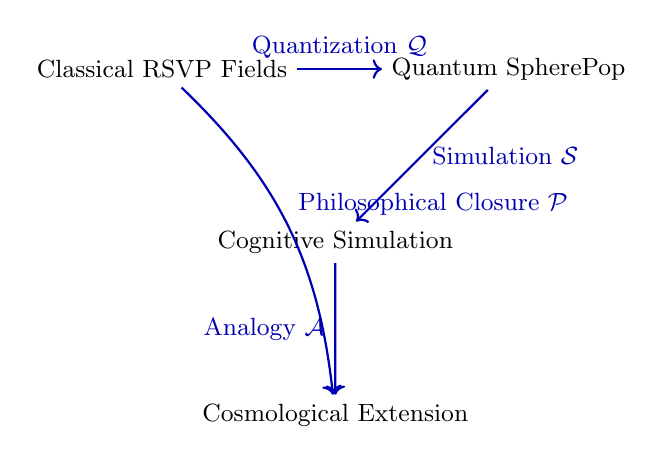
\begin{tikzpicture}[scale=1.1, every node/.style={font=\small}]
\node (A) at (0,0) {Classical RSVP Fields};
\node (B) at (4,0) {Quantum SpherePop};
\node (C) at (2,-2) {Cognitive Simulation};
\node (D) at (2,-4) {Cosmological Extension};
\draw[->,thick,blue!70!black] (A) -- (B) node[midway,above]{Quantization $\mathcal{Q}$};
\draw[->,thick,blue!70!black] (B) -- (C) node[midway,right]{Simulation $\mathcal{S}$};
\draw[->,thick,blue!70!black] (C) -- (D) node[midway,left]{Analogy $\mathcal{A}$};
\draw[->,thick,blue!70!black,bend left=20] (A) to node[above right]{Philosophical Closure $\mathcal{P}$} (D);
\end{tikzpicture}
\captionof{figure}{Conceptual evolution of RSVP theory from classical cognition to cosmological entropic equilibrium.}
\end{center}

\subsection{Summary}\label{sec:I-summary}
Appendix~I consolidates the speculative frontier of the Quantum SpherePop program.  
It enumerates formal conjectures, computational and experimental objectives, and philosophical generalizations linking mind and cosmos under a single entropic symmetry.  
Progress on any of these fronts—particularly proof of Conjectures~\ref{conj:I-clio}--\ref{conj:I-tqft}—would advance the mathematical and empirical foundations of RSVP theory and its unification of cognition, physics, and meaning.


%==================== Bibliography ====================
\begin{thebibliography}{99}

\bibitem{Evans2010} Evans, L. C. (2010). \emph{Partial Differential Equations}. AMS.

\bibitem{Kuramoto1984} Kuramoto, Y. (1984). \emph{Chemical Oscillations...}. Springer.

\bibitem[Penrose(1977)]{Penrose1977}
Penrose, R. (1977).
\emph{The Large, the Small and the Human Mind}.
Cambridge University Press.

\bibitem[Kuramoto(1984)]{Kuramoto1984}
Kuramoto, Y. (1984).
\emph{Chemical Oscillations, Waves, and Turbulence}.
Springer.

\bibitem[Villain(1975)]{Villain1975}
Villain, J. (1975).
``Theory of One-Dimensional and Two-Dimensional Magnets with an Easy Magnetization Plane.''
\emph{Journal de Physique}, 36(6), 581–590.

\bibitem[Bott \& Tu(1982)]{BottTu1982}
Bott, R., \& Tu, L. W. (1982).
\emph{Differential Forms in Algebraic Topology}.
Springer.

\bibitem[Zinn-Justin(2002)]{ZinnJustin2002}
Zinn-Justin, J. (2002).
\emph{Quantum Field Theory and Critical Phenomena}.
Oxford University Press.

\bibitem[Witten(1988)]{Witten1988}
Witten, E. (1988).
``Topological Quantum Field Theory.''
\emph{Communications in Mathematical Physics}, 117(3), 353–386.
\end{thebibliography}

\end{spacing}
\end{document}

